\section{External Interface Requirements}
The following mockups provide a model of the graphic interface provided by the system. \\
We will create a user interface that will be user friendly in order to be easy to use also from non-technical users. \\
The mockups has the aim to illustrate the main aspects of the CLup and CLup operator.
\subsection{User Interfaces (CLup)}
The development of CLup app aims to have a easy-to-use interface for User who has a Smartphone. In particular the application have to be intuitive and reliable in order to give Users the possibility to book an appointment without any obstacles.\\
The following mockups show the main operation allowed by Clup to the Smart User:
\begin{figure}[h]
  \caption{Login: Users already registered signes in with their credential.}
  \label{fig: Login}
  \centering
  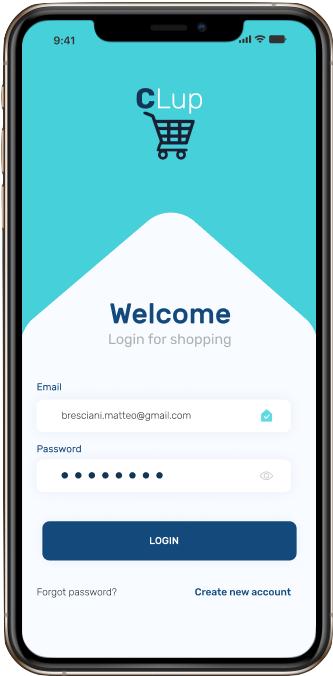
\includegraphics[scale=0.35]{images/mockup/login.png}
\end{figure}
\begin{figure}[H]
  \caption{Market selection: After the login, the user have to select in which market wants to go shopping, due to his position.}
  \label{fig:Login}
  \centering
 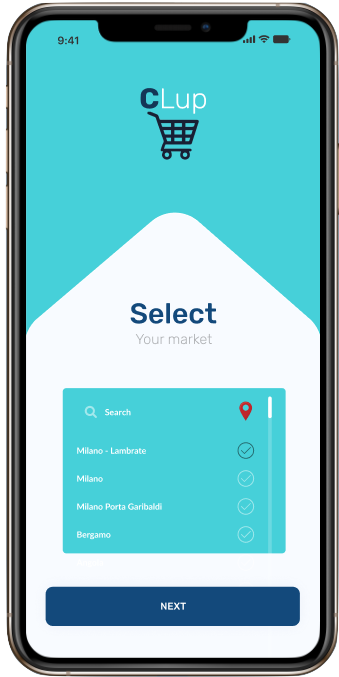
\includegraphics[scale=0.31]{images/mockup/select2.png}

\end{figure}







\begin{figure}[H]
  \centering
  \subfloat[Page 1.]{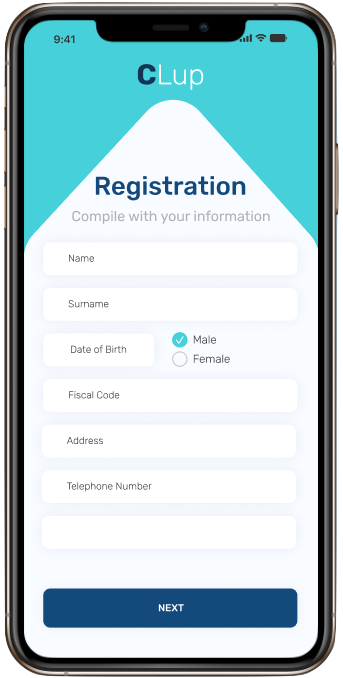
\includegraphics[scale=0.260]{images/mockup/reg1.png}\label{fig:f1}}
  \hfill
  \subfloat[Page 2.]{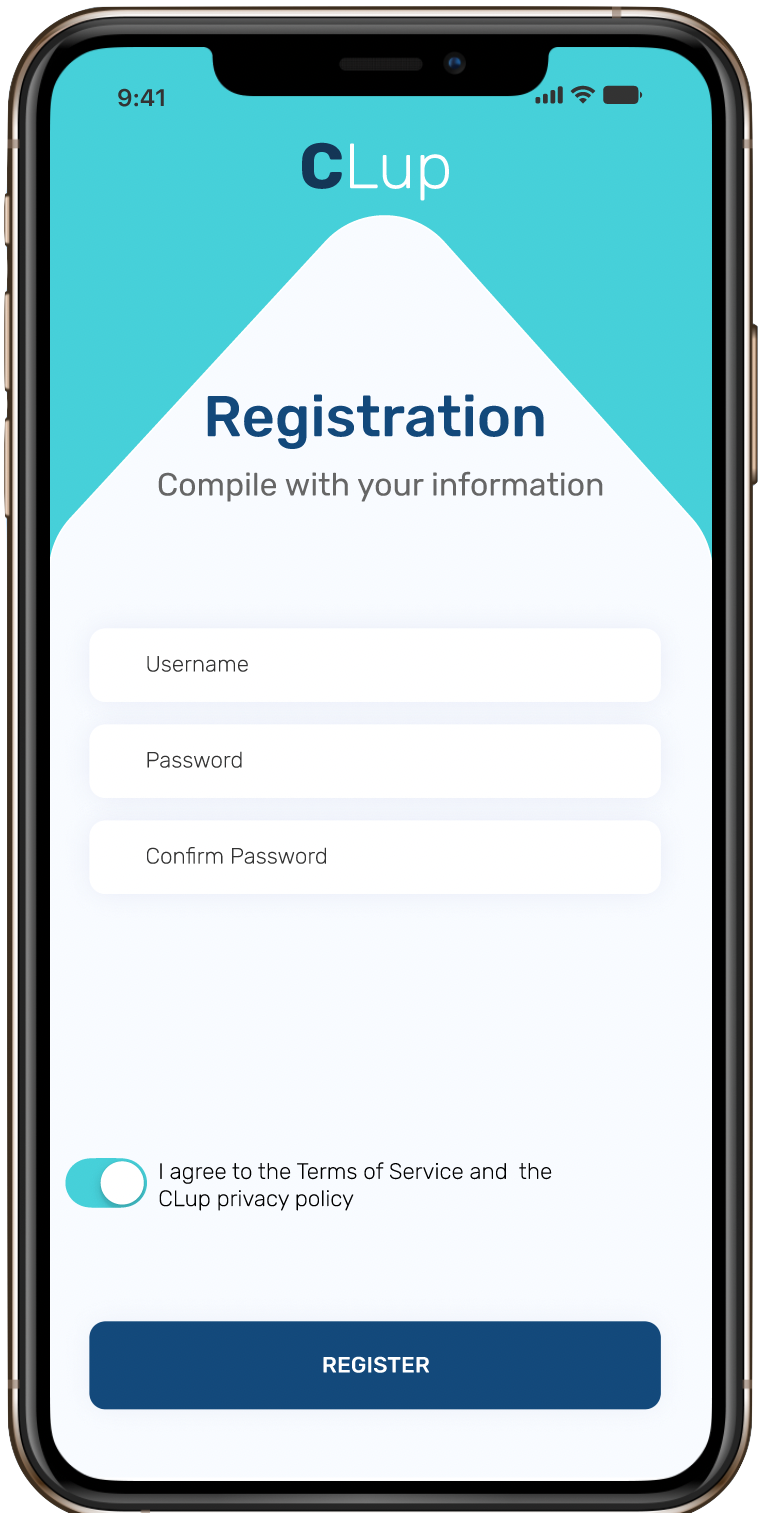
\includegraphics[scale=0.260]{images/mockup/reg2.png}\label{fig:f2}}
  \caption{Registration: Users not registered can sign up himself putting his own data, e-mail and password. In addition Users have to accepts the Term of Service and the CLup privacy policy to proceed.}
\end{figure}
\begin{figure}[H]
 
  \label{fig:Home}
  \centering
  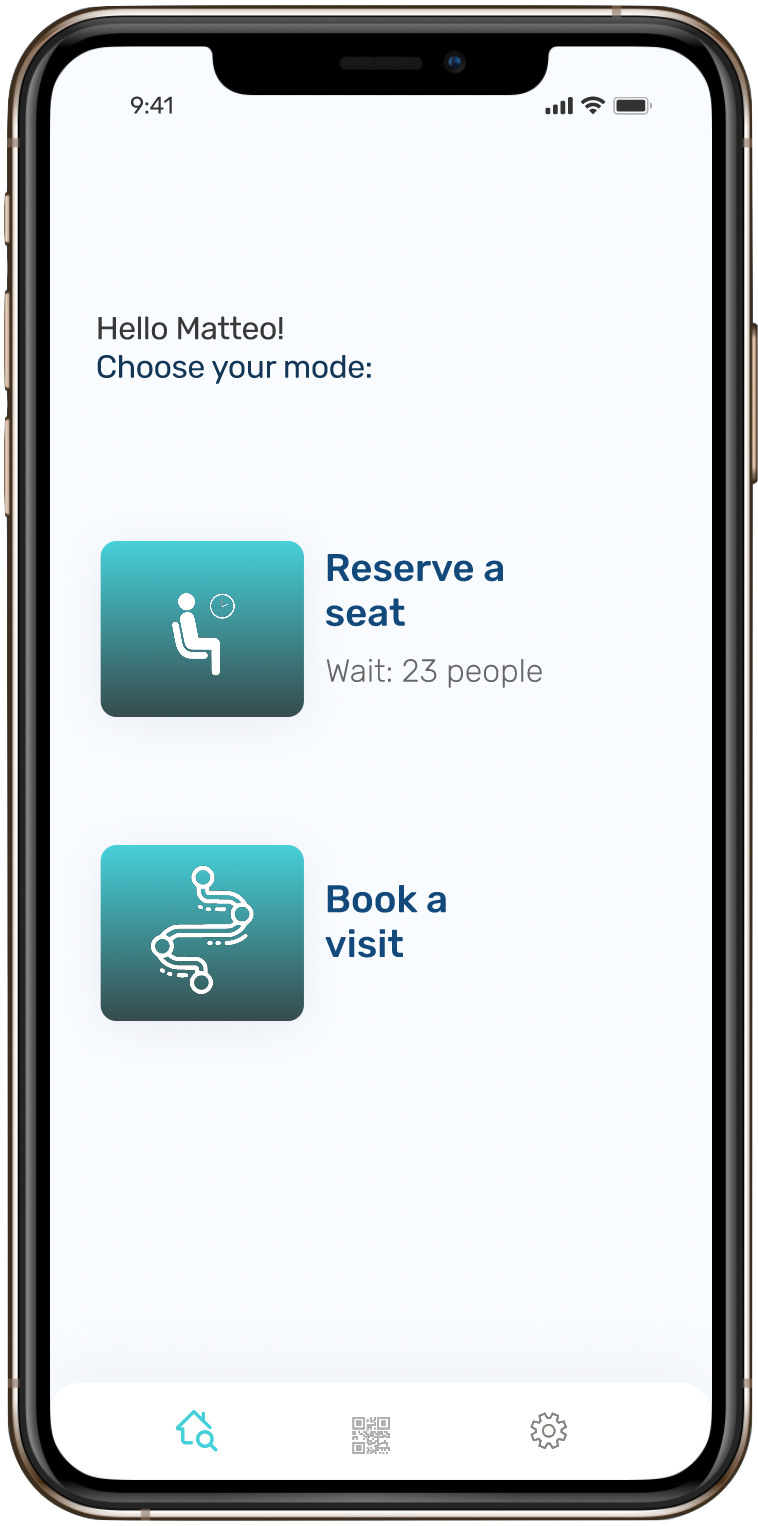
\includegraphics[scale=0.26]{images/mockup/home1.png}
   \caption{Home: Homepage of CLup from which the User can select to book a Visit or a Reservation.}

\end{figure}
\begin{figure}[H]
    
     \begin{center}

        \subfloat[User chooses Reservation.]{%
            \label{fig:first}
            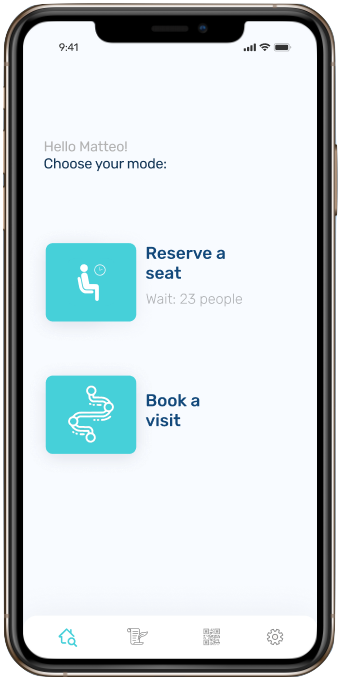
\includegraphics[scale=0.30]{images/mockup/reserve1.png}
        }%
        \subfloat[Shopping size selection.]{%
           \label{fig:second}
           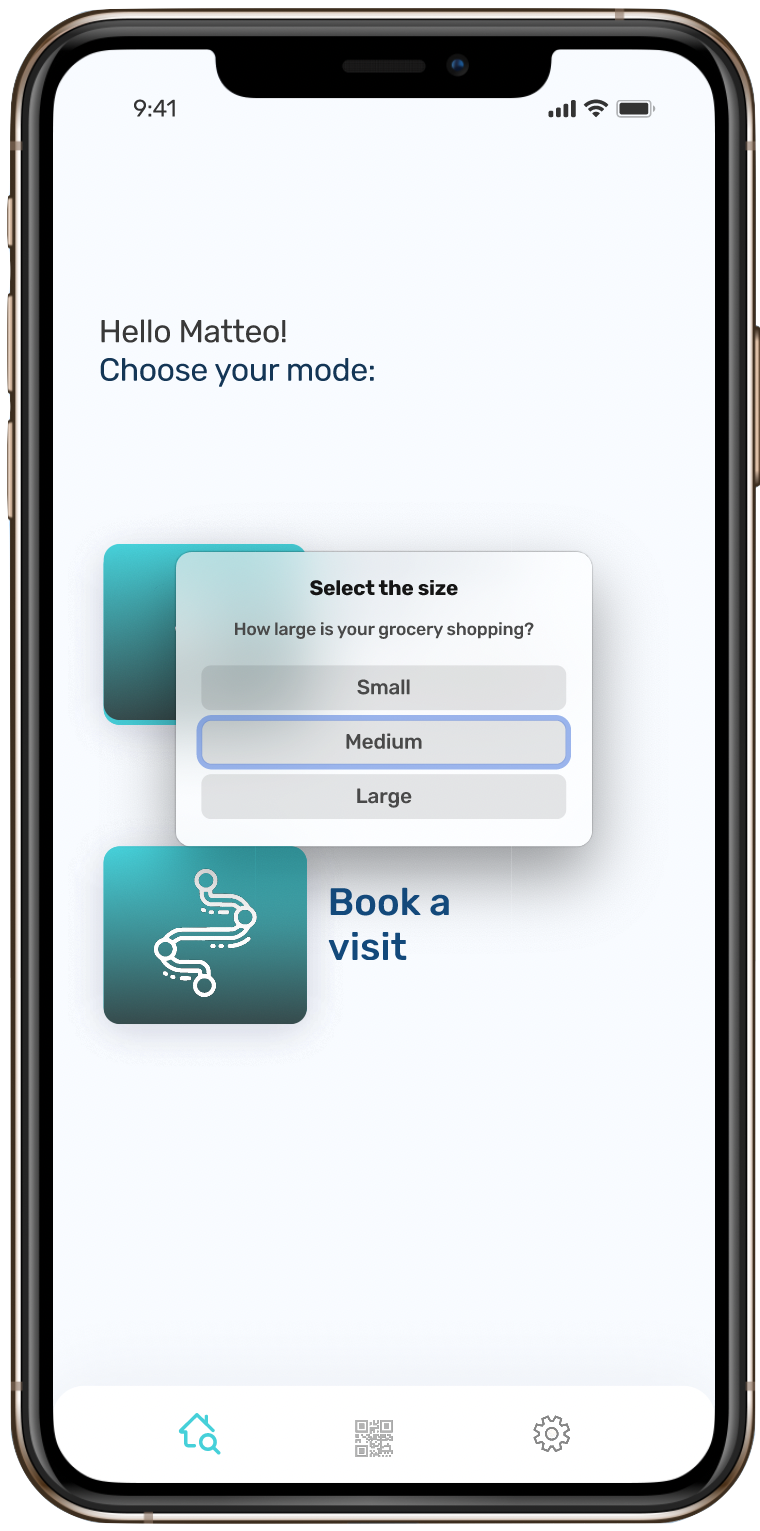
\includegraphics[scale=0.30]{images/mockup/reservation_size.png}
        }\\ %  ------- End of the first row ----------------------%
        \subfloat[Booking confirm.]{%
            \label{fig:third}
            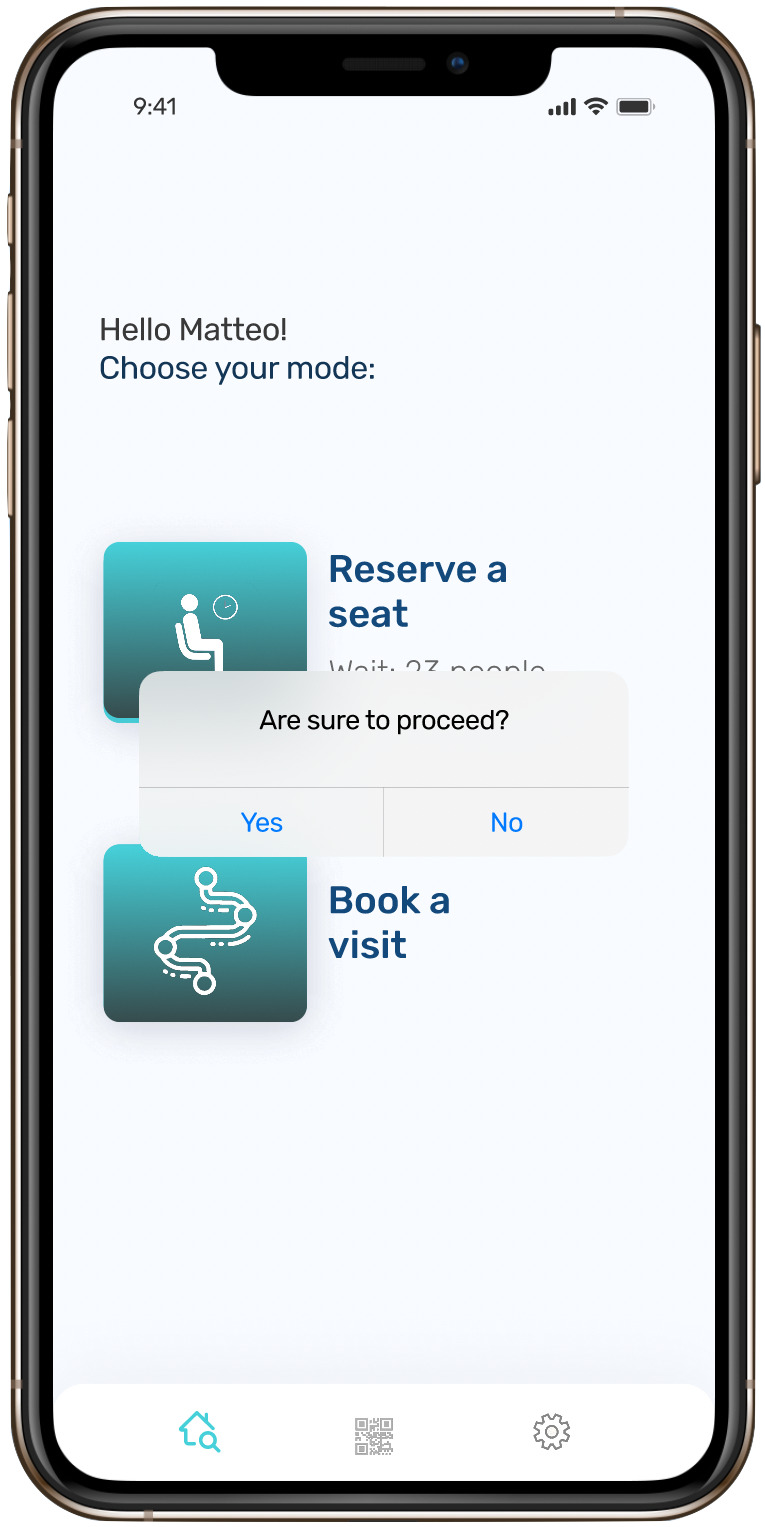
\includegraphics[scale=0.30]{images/mockup/reserve2.png}
        }%
        \subfloat[Reservation's QRCode.]{%
            \label{fig:fourth}
            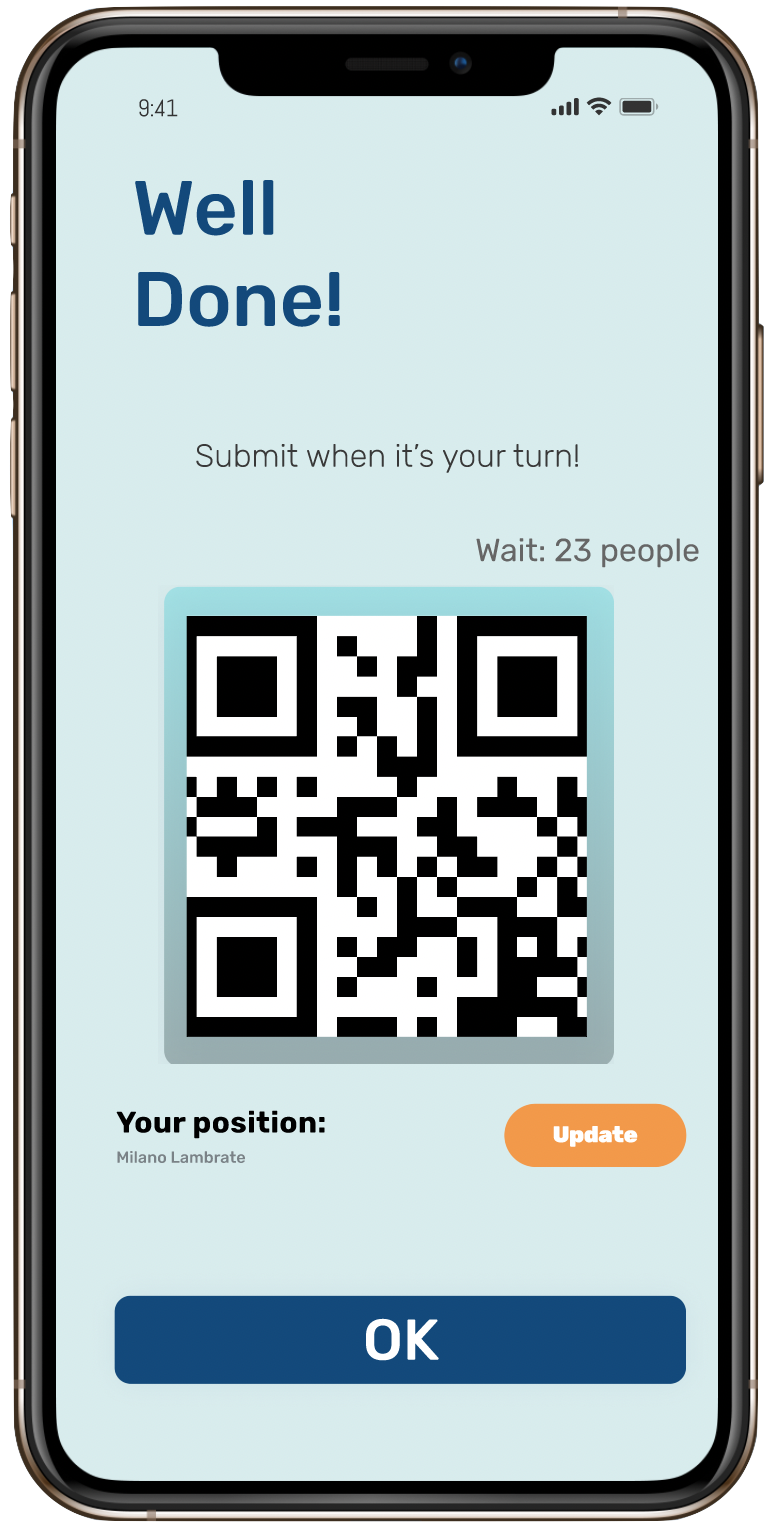
\includegraphics[scale=0.30]{images/mockup/qrcode_reservation_done.png}
        }
%
    \end{center}
    \caption{Reservation: The Smart User can book a Reservation with the following steps.}
   \label{fig:subfigures}
\end{figure}

\begin{figure}[H]
     \begin{center}
%
        \subfloat[Smart User chooses Visit]{%
            \label{fig:first}
            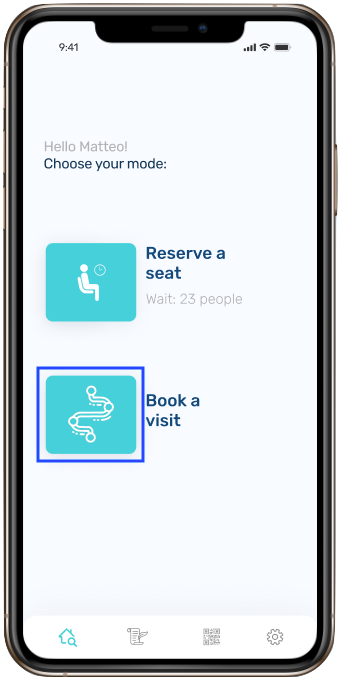
\includegraphics[scale=0.30]{images/mockup/visit00.png}
        }%
        \subfloat[Date selection.]{%
           \label{fig:second}
           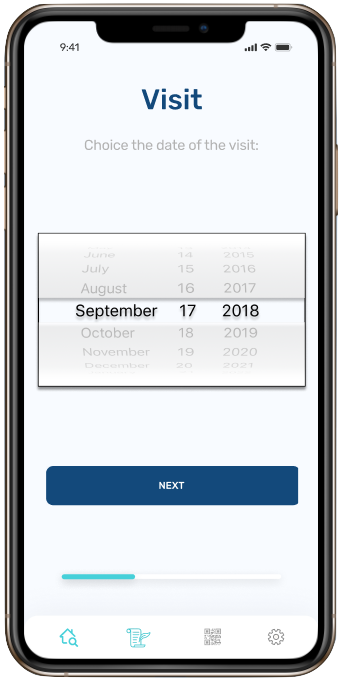
\includegraphics[scale=0.30]{images/mockup/visit1.png}
        }\\ %  ------- End of the first row ----------------------%
        \subfloat[Time period selection.]{%
            \label{fig:third}
            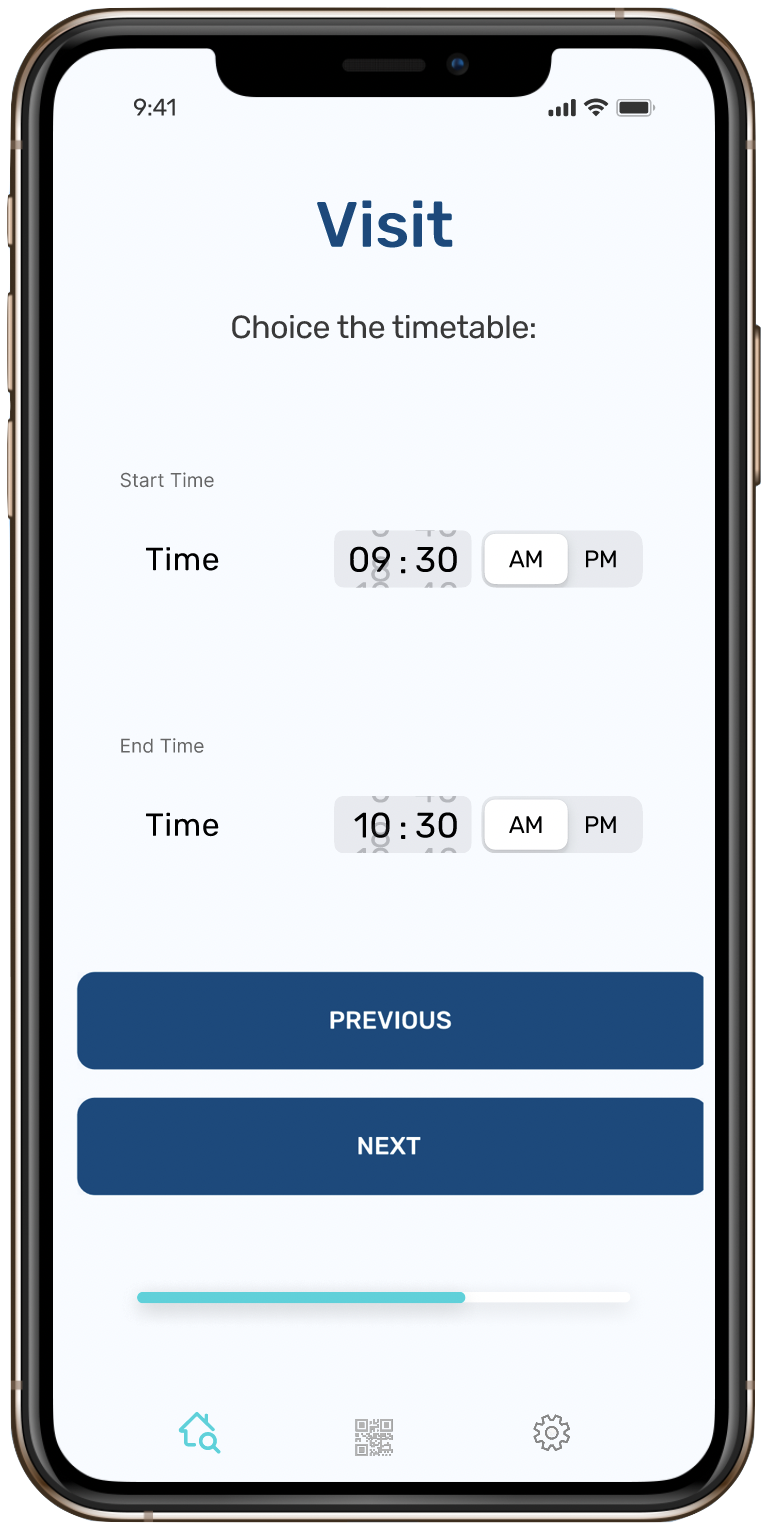
\includegraphics[scale=0.30]{images/mockup/visit2.png}
        }%
        \subfloat[Shopping size selection.]{%
            \label{fig:fourth}
            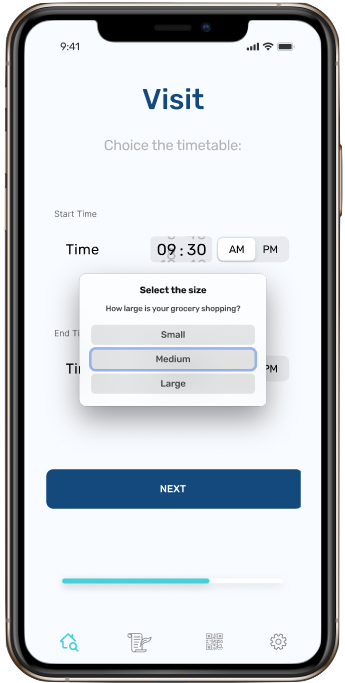
\includegraphics[scale=0.30]{images/mockup/visit_size.png}
        }%
%
    \end{center}
    \caption{%
       Visit: The Smart User can book a Visit with the following steps. At the end Visit's QRCode is provided.
     }%
   \label{fig:subfigures}
\end{figure}



\begin{figure}[H]

     \begin{center}
%
        \subfloat[Only Reservation booked.]{%
            \label{fig:first}
            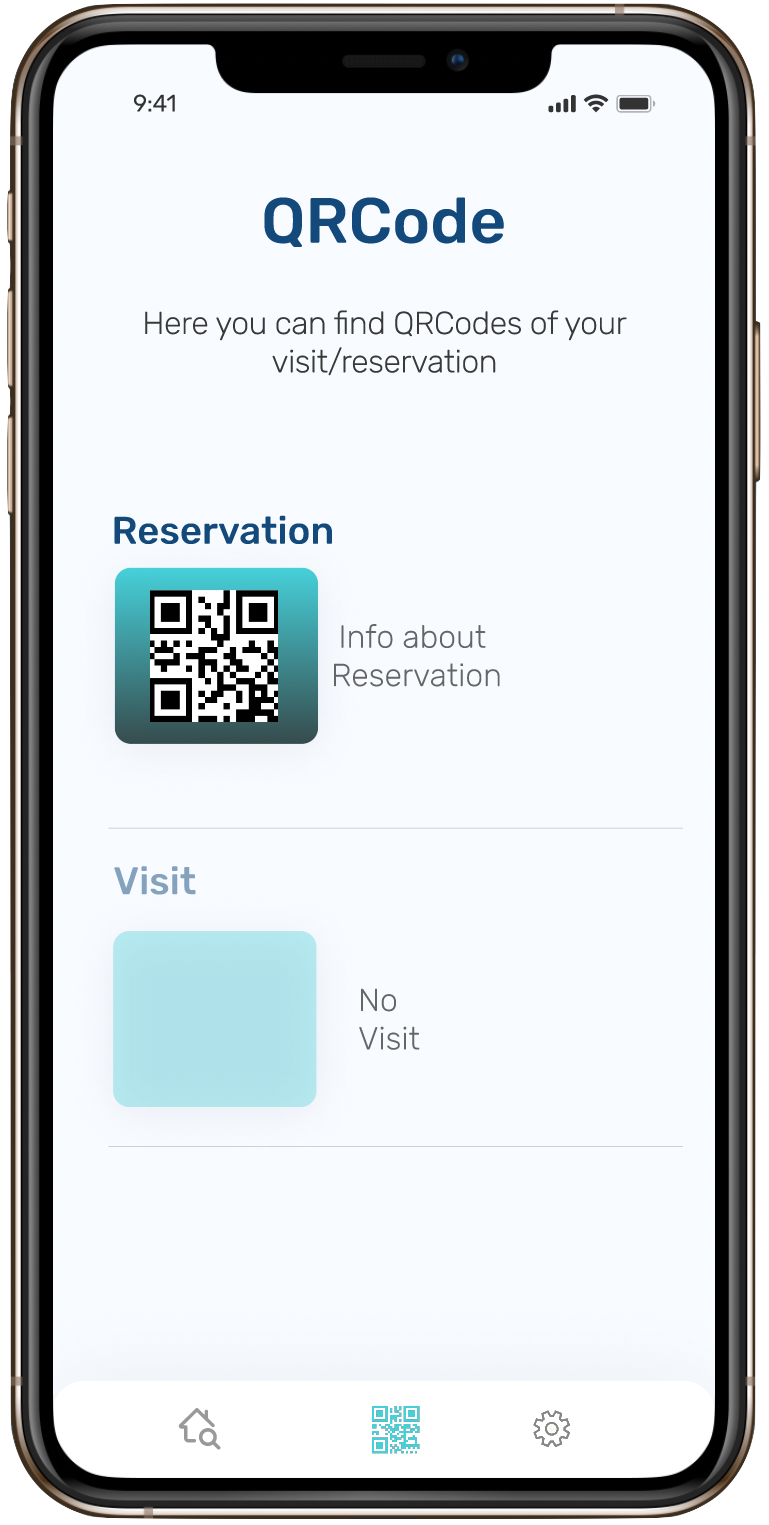
\includegraphics[scale=0.30]{images/mockup/qr2.png}
        }%
        \subfloat[Visit and Reservation booked.]{%
           \label{fig:second}
           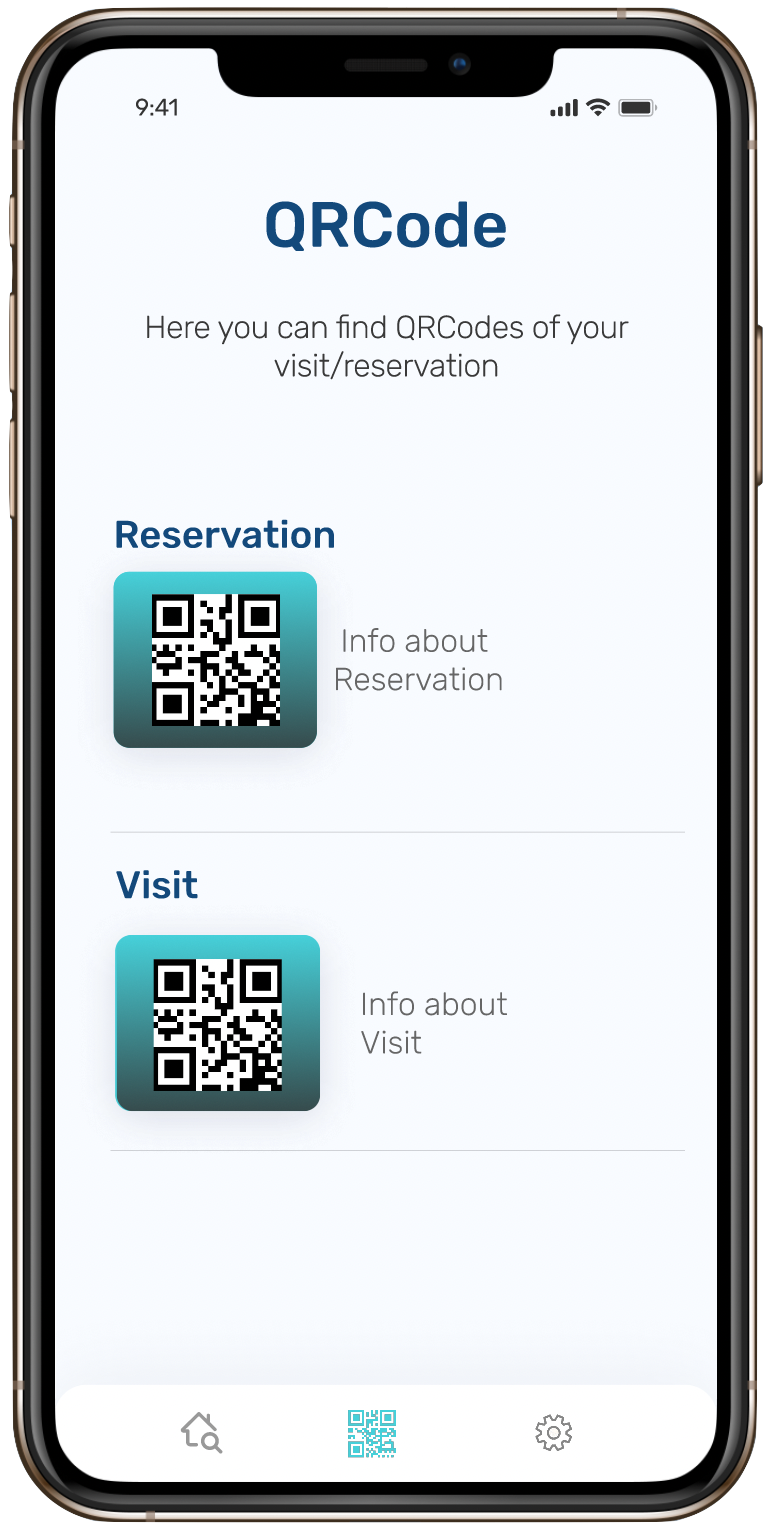
\includegraphics[scale=0.30]{images/mockup/qr4.png}
        }\\ %  ------- End of the first row ----------------------%
        \subfloat[Smart User swipes left.]{%
            \label{fig:third}
            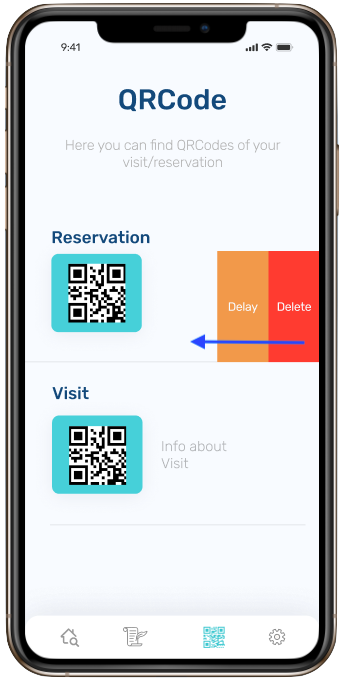
\includegraphics[scale=0.30]{images/mockup/qr5.png}
        }%
        \subfloat[Booking's QRCode.]{%
            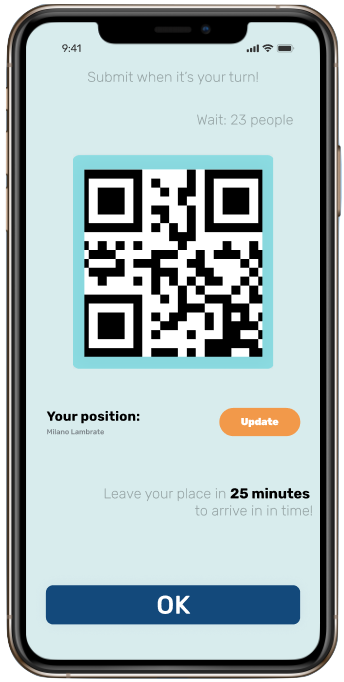
\includegraphics[scale=0.30]{images/mockup/qr_reservation.png}
        }%
%
    \end{center}
    \caption{
        QRCode section: the User can manage his booking. A Smart User can cancel, delay (only for Reservation), or visualize his QRCode in order to access to the market.
     }
   \label{fig:subfigures}
\end{figure}


\begin{figure}[H]
  \centering
  \subfloat[Delay confirmation of a Reservation]{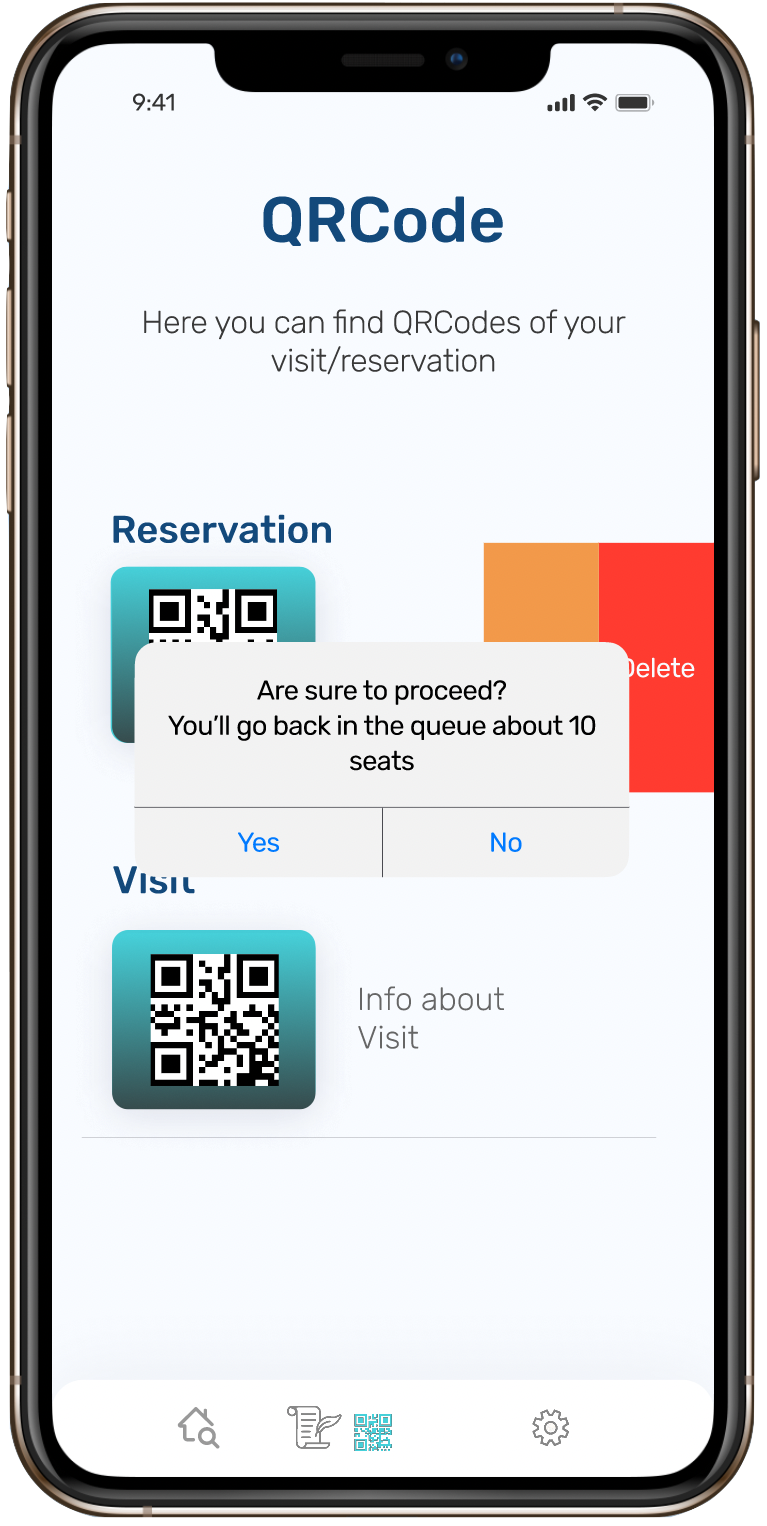
\includegraphics[scale=0.30]{images/mockup/qr1.png}\label{fig:f1}}
  \hfill
  \subfloat[Cancellation confirmation of a Visit]{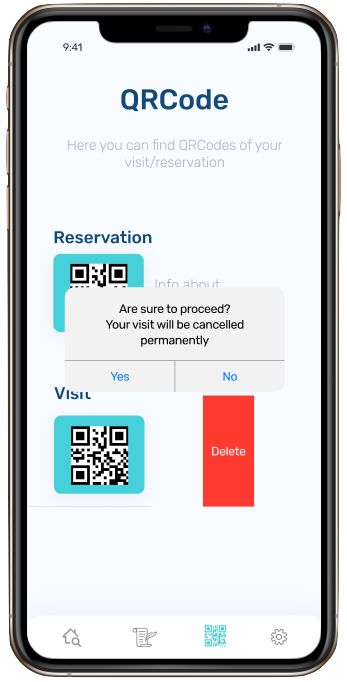
\includegraphics[scale=0.30]{images/mockup/qr7.png}\label{fig:f2}}
  \caption{Cancel and Delay action: A alert will be shown to Smart User to confirm his action.}
\end{figure}



\begin{figure}[H]
  \centering
  \subfloat[A notification is sent to a Smart User to inform him to leave in order to reach the market in time.]{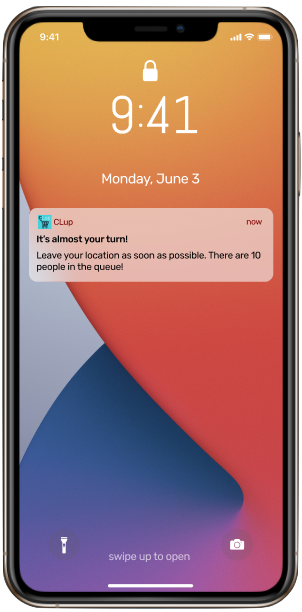
\includegraphics[scale=0.50]{images/mockup/notify1.png}\label{fig:f1}}
  \hfill
  \subfloat[An SMS is sent to a Mobile User with booking information of his Visit. In particular contains the Booking's schedule and the Identification Code to submit.]{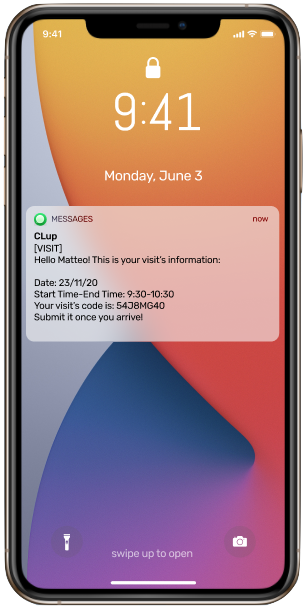
\includegraphics[scale=0.50]{images/mockup/visit_SMS.png}\label{fig:f2}}
  \caption{Notification and SMS: User receive his information about his Booking depending on whether is a Smart or Mobile User.}
\end{figure}

\pagebreak

\subsection{Receptionist Interfaces (CLup Operator)}
\textbf{CLup Operator}, the desktop app, is introduced to give Users who has no Smartphone the possibility to book an appointment at the market. Mobile Users have to call a Receptionist through a customer service number.\\
The Receptionist so aims to interact between the User and the system in order to manage his appointment, acting like an intermediary.
Even this application must be simple, in order to allow Receptionist to interact with Mobile User in a proper and effective way.\\
The following mockups show the main operation allowed by Receptionist through his application to manage Booking of the Mobile Users.
\begin{figure}[H]
  \caption{Receptionist signes in with their credential.}
  \label{fig:Login}
  \centering
  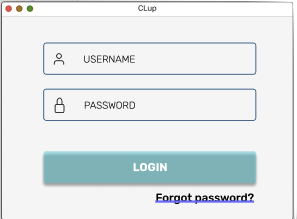
\includegraphics[scale=0.55]{images/mockup/LOGIN_REC.png}

\end{figure}

\begin{figure}[H]
  \caption{Receptionist can register a new Mobile User or select a new one if it's already registered.}
  \label{fig:Login}
  \centering
  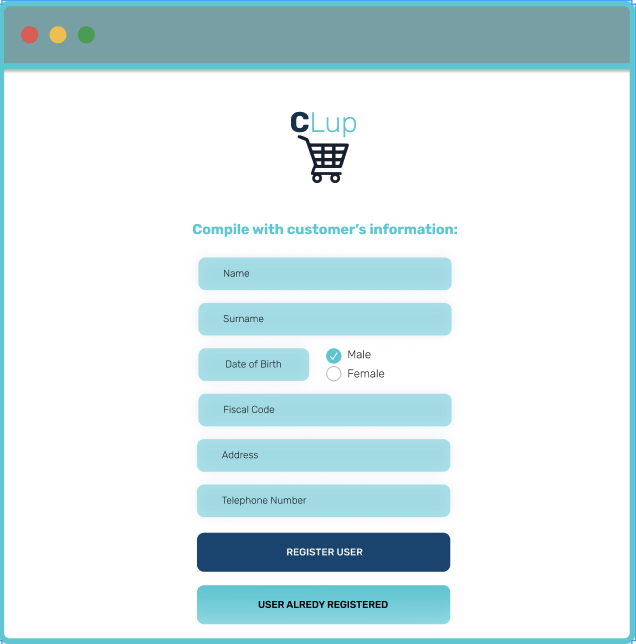
\includegraphics[scale=0.32]{images/mockup/LOGREG.png}

\end{figure}

\begin{figure}[H]
  \caption{Receptionist selects the Mobile User already registered.}
  \label{fig:Login}
  \centering
  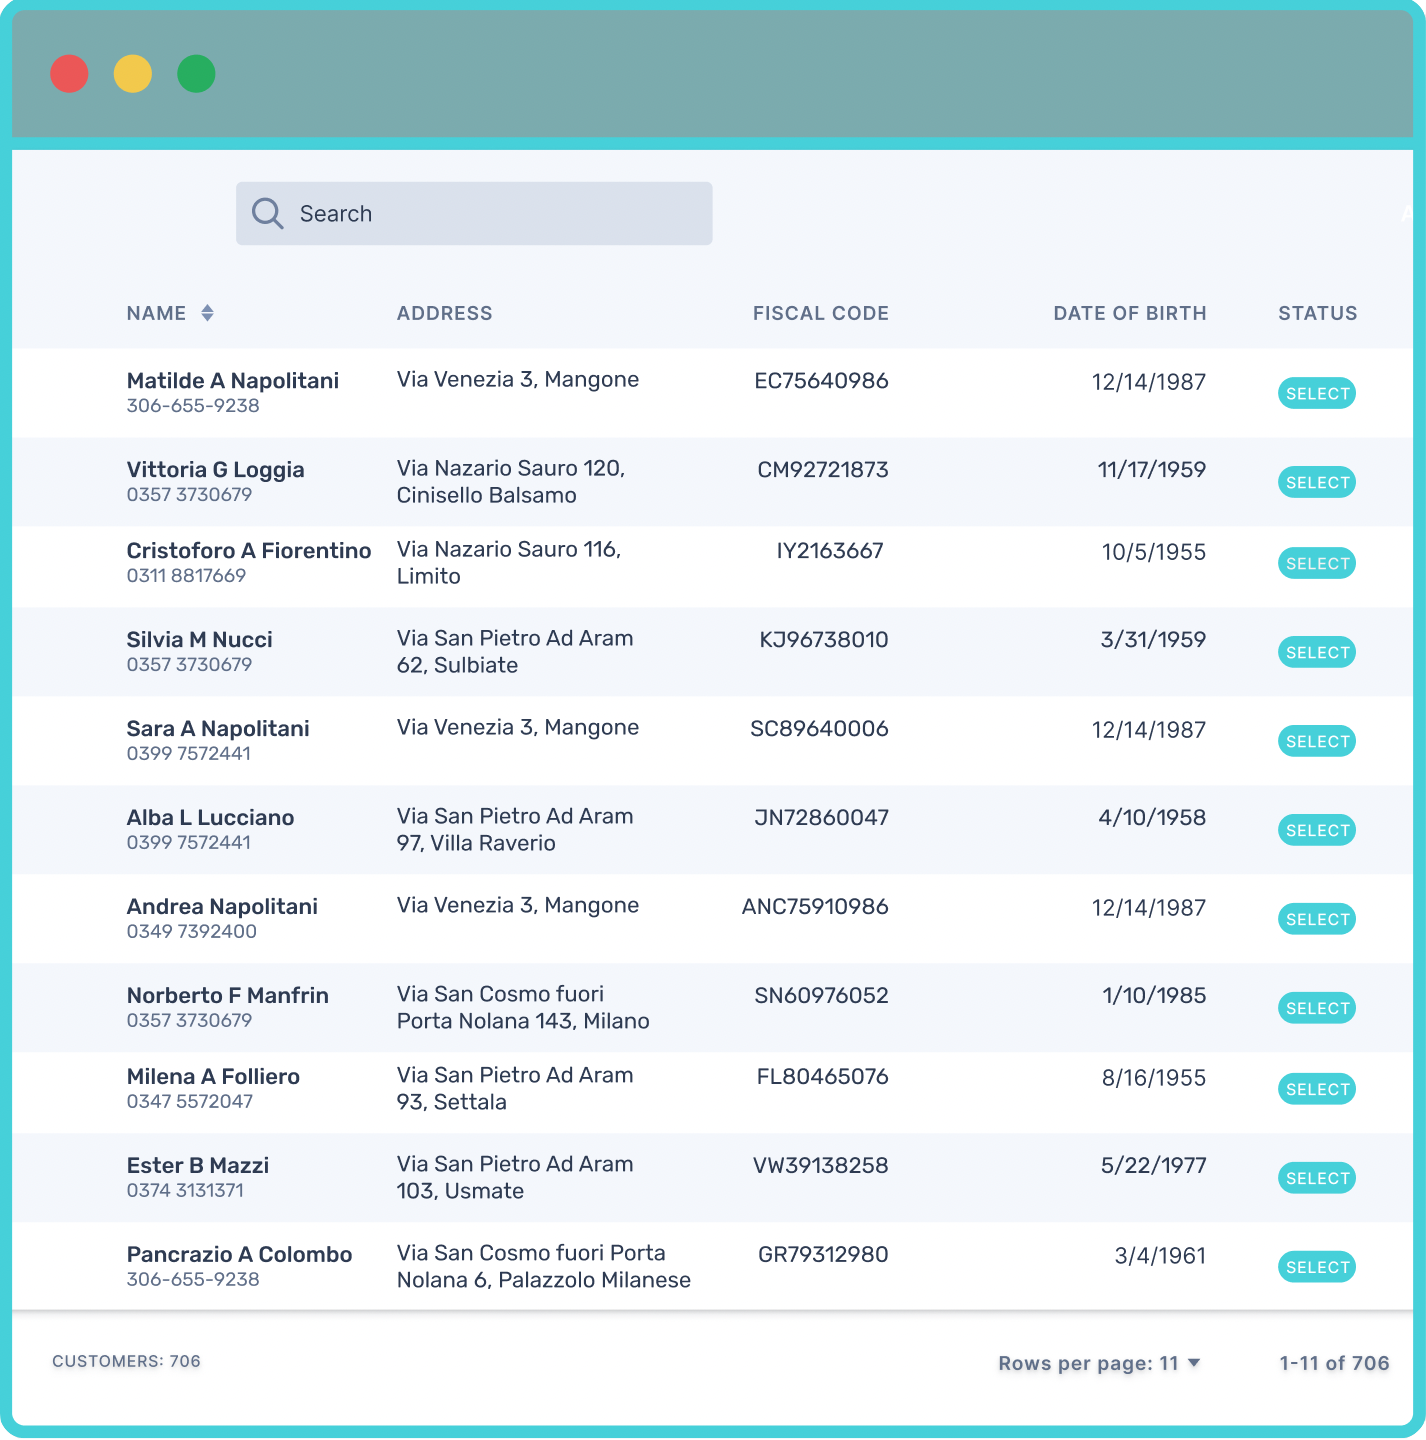
\includegraphics[scale=0.32]{images/mockup/Select_User.png}

\end{figure}

\begin{figure}[H]
  \caption{Receptionist can manage Mobile User's Booking.}
  \label{fig:Login}
  \centering
  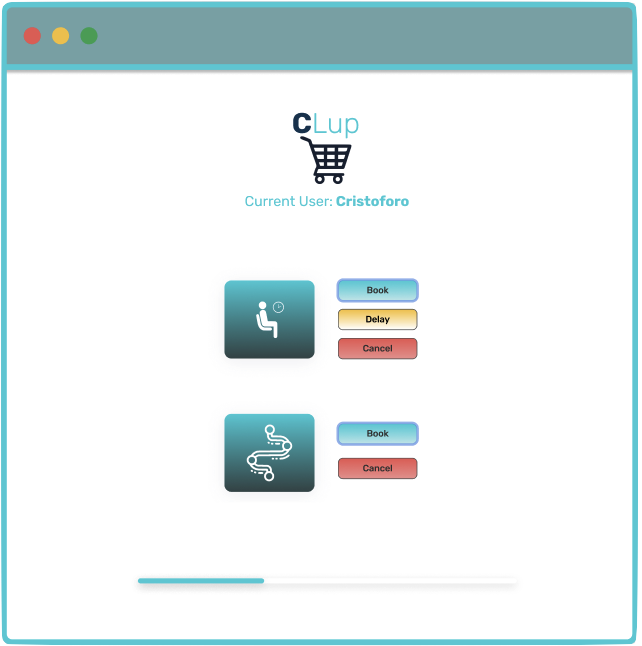
\includegraphics[scale=0.32]{images/mockup/Home_Rec.png}

\end{figure}


\begin{figure}[H]
  \caption{Receptionist selects the grocery shopping size told by Mobile User.}
  \label{fig:Login}
  \centering
  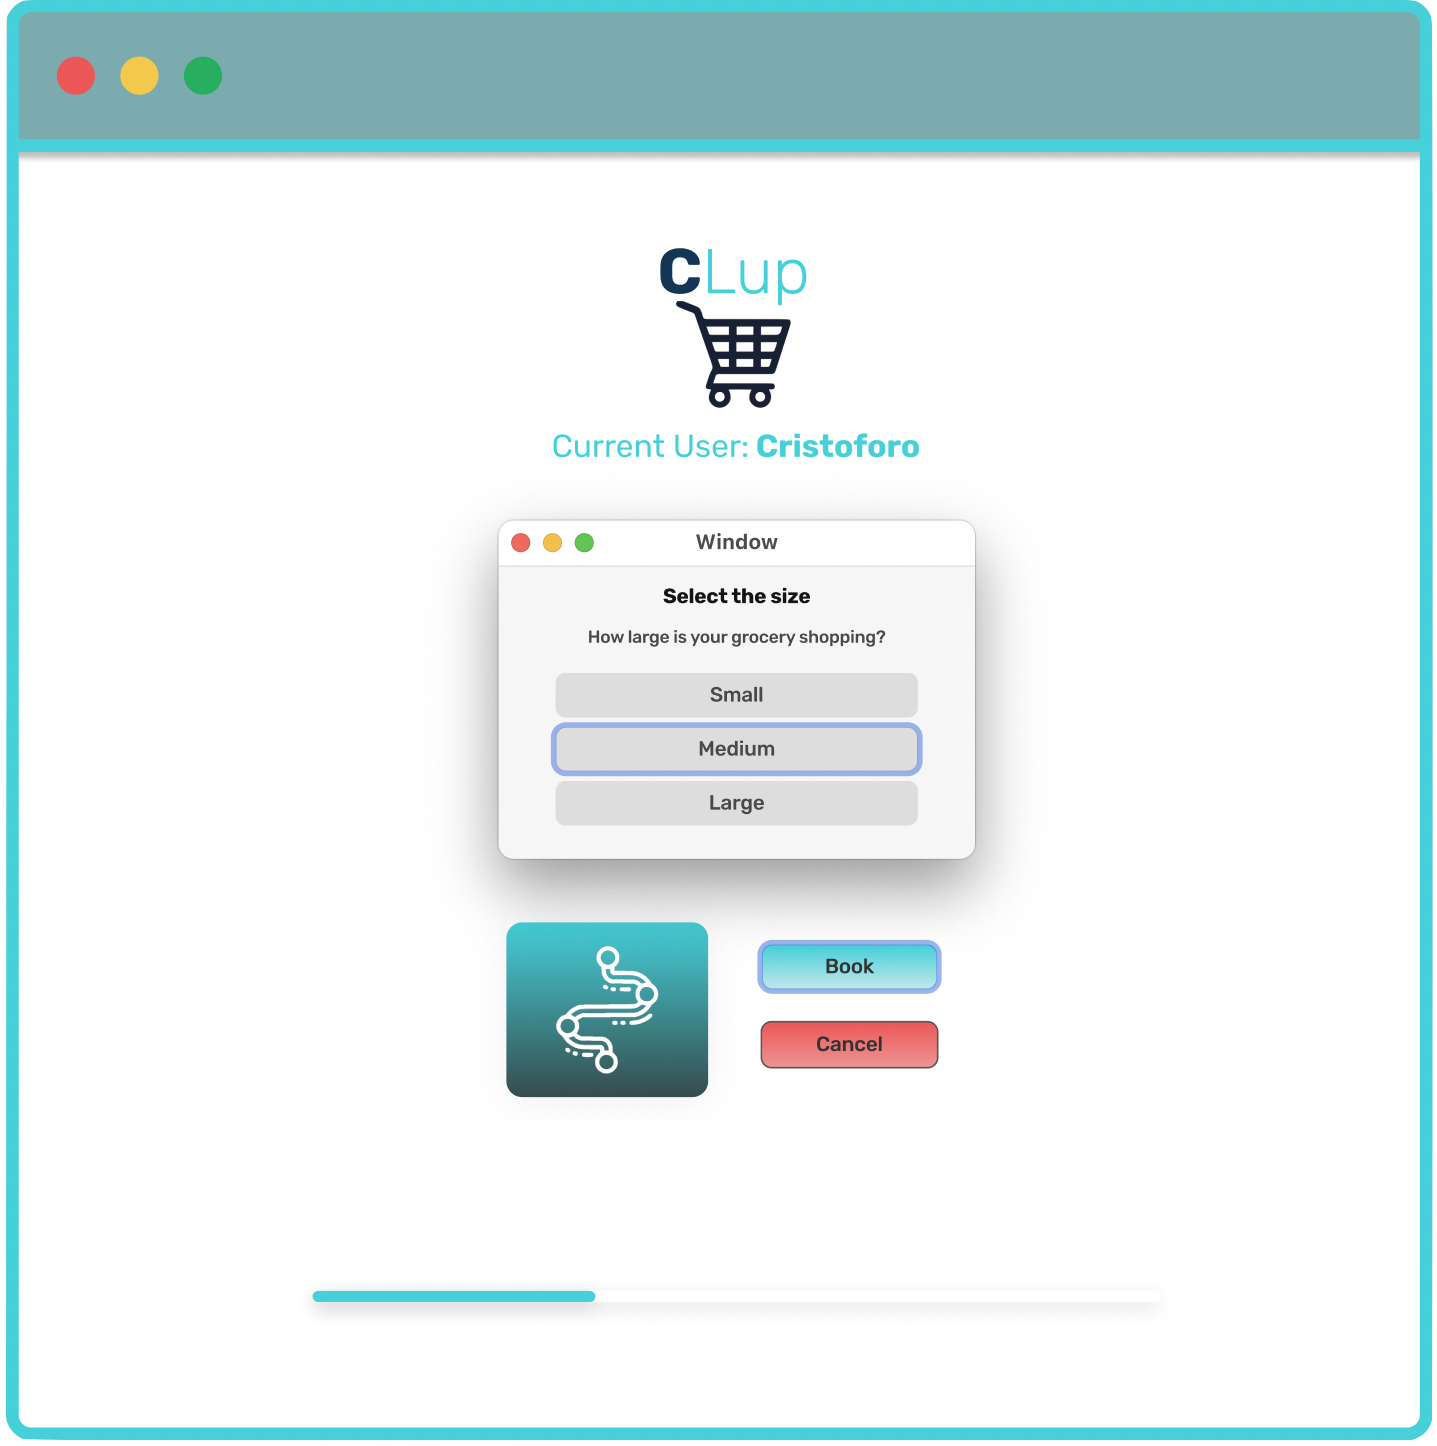
\includegraphics[scale=0.31]{images/mockup/Size_Rec.png}

\end{figure}


\begin{figure}[H]
  \caption{Receptionist inserts visit information told by Mobile User.}
  \label{fig:Login}
  \centering
  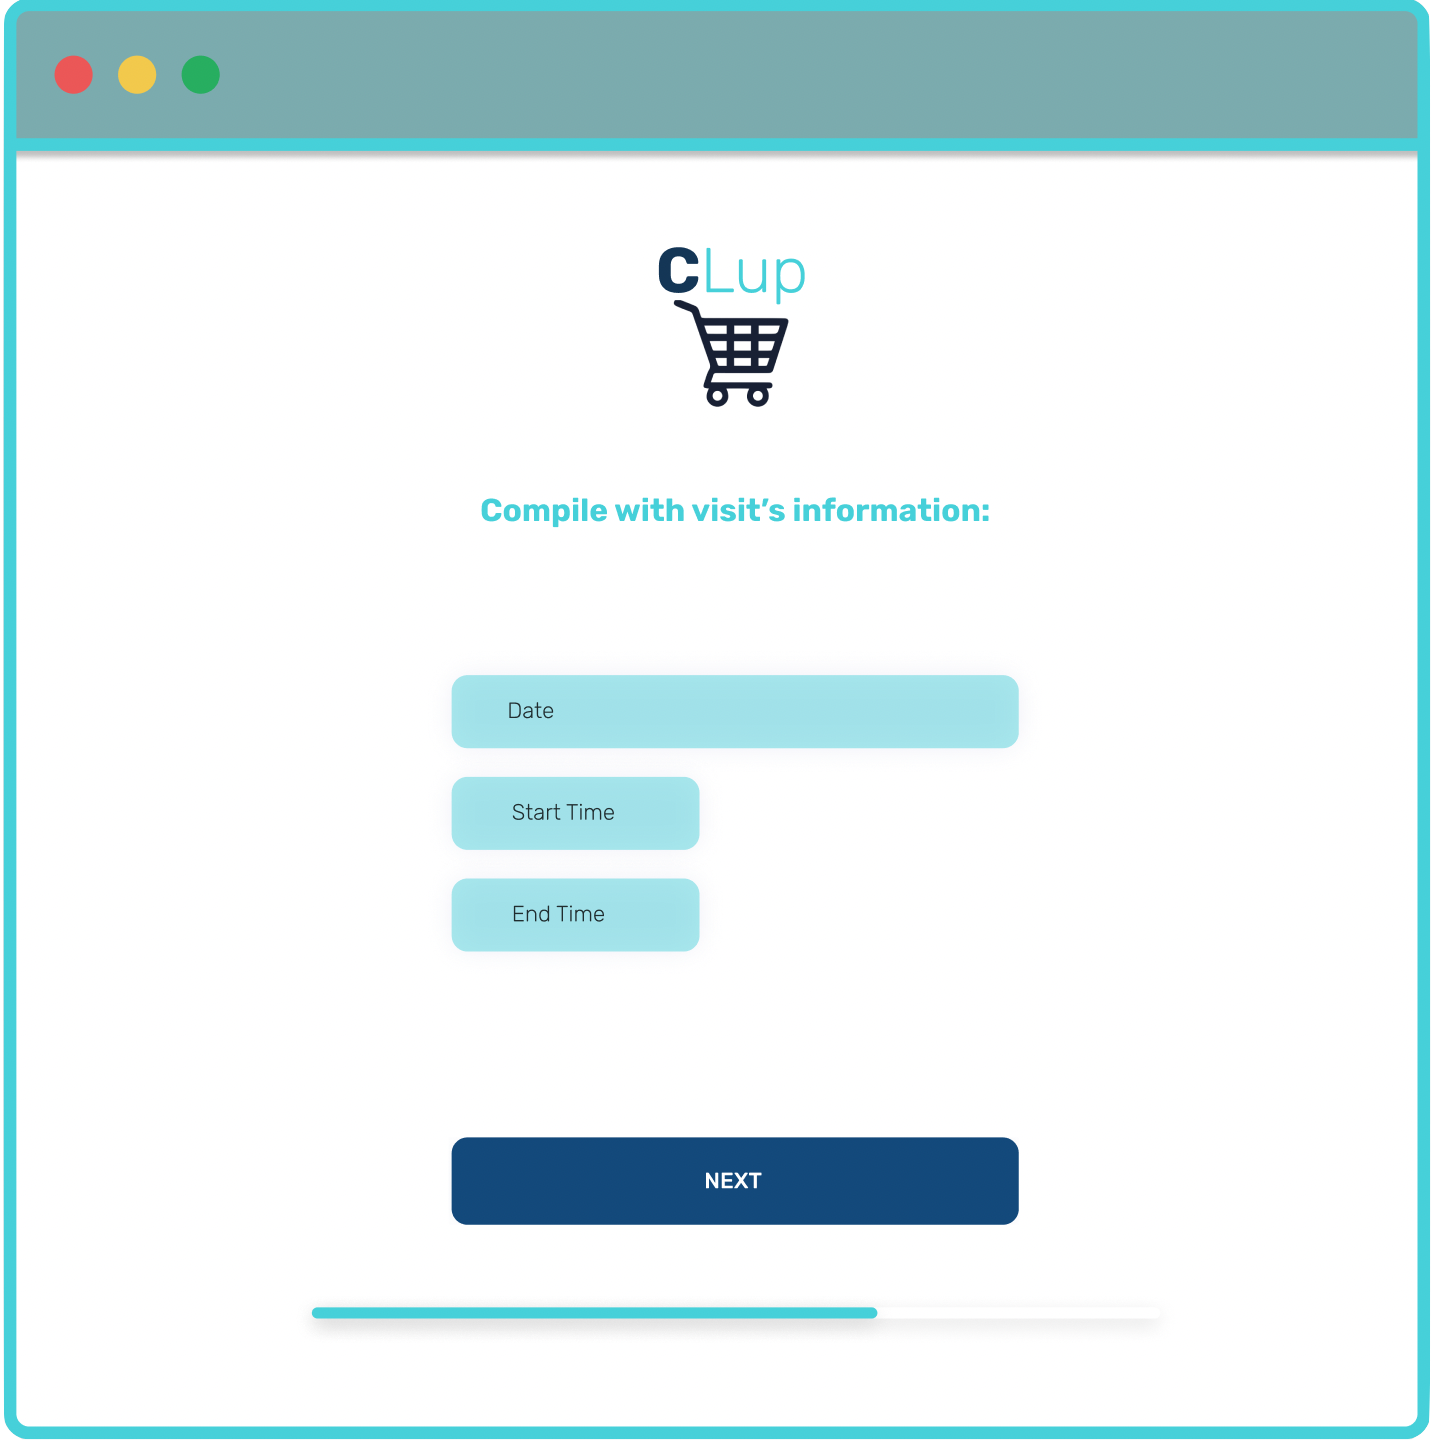
\includegraphics[scale=0.31]{images/mockup/info_visit_rec.png}

\end{figure}

\begin{figure}[H]
  \caption{Booking made by Receptionist is finished.}
  \label{fig:Login}
  \centering
  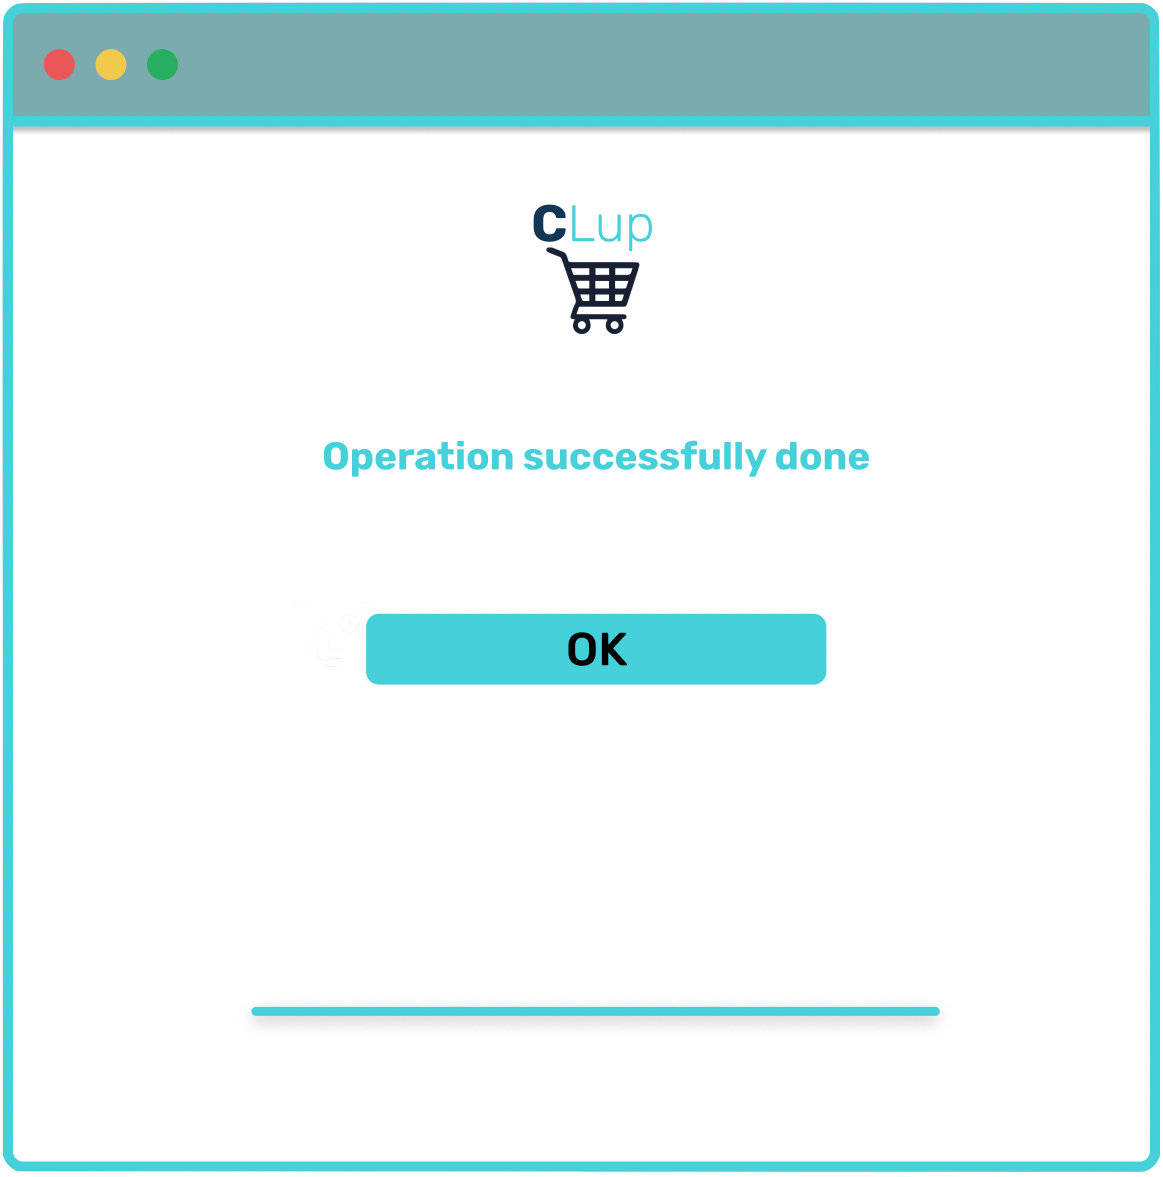
\includegraphics[scale=0.25]{images/mockup/Done_Rec.png}

\end{figure}
\par
\subsection{Hardware Interfaces}
The supermarket will have two scanners associated to an employee's device in order to validate the booking:

\par \medskip 
\begin{itemize}
\item One at the entry, that will read QR code and will confirm client reservations in case they will be valid. \\
The scanner will reject reservation if QR code will result invalid or will have passed to much time from its call.
\item One at the exit, that when clients will finish shopping allow them to exit to supermarket opening the doors. \\
Another usage of exit QR code is to monitor the numbers of client into the shop.
\end{itemize} 
\par \medskip 
The scanners will be used to obtain information about client shopping time.

\subsection{Software Interfaces}
CLup notices User when leave in order to reach the market in time also thanks to Google Maps APIs. Infact CLup use them in order to determine how much time a User have to put due to his position.
The choice of using Google Maps APIs derives from the easy usability, frequency update and very large documentation.
The system, in addition to CLup and CLup Operator application doesn't use any external interfaces.


\subsection{Communication Interfaces}
Every User uses a HTTPS protocol to make request to CLup's servers. In this way informations sent are safe due to encryption provided by the TLS protocol. The same is used by Receptionist to communicate with the server.

\pagebreak

\section{Functional Requirements}
\begin{description}
    \item[G1]User enters once arrived at the market.
    
    \begin{description}
    \item[R1] Smart User can receive the first notification to reach the market; 
    \item[R2] Mobile User can receive an SMS needed to enter / exit from the market;   %-- 
    \item[R3] The system provide the time estimation to reach the market;
    \item[R4] The User chooses the startTime / endTime of the Visit;
    \item[R5] The User can postpone his turn by 10 turns;
    \item[R8] The system provides the number Users in queue; %--
    \item[D1] The system can delete the Reservation when the Smart User accumulates a delay to reach the market greater than 10 minutes; 
    \item[D2] The system can delete the Reservation the Mobile User accumulates a delay to reach the market greater than 15 minutes; 
    \item[D3] The system handles the threshold number of Users allowed in the market
    \item[D4] The Smart User have to be connected to Internet through Wi-Fi/Cellular network
    \item[D5] The Mobile User have to be connected to his own mobile operator
    \item[D6] A Visit is associated to a Date and a period of time (start/end time); 
    \item[D7] A booking is associated to one and only one QRCode;  
    \end{description}
    
    \item[G2]Put a limit to the number of Users in the market.
    
    \begin{description}
    \item[R4] The User chooses the startTime / endTime of the Visit;
    \item[R6] The system allows the User to enter/exit from the market with the QRCode submission; 
    \item[R7] The system store the enter/exit time from the market after the QRCode submission; 
    \item[D3] The system handles the threshold number of Users allowed in the market;
    \end{description}
    
    \item[G3]Smart User can make a Reservation of a seat in the market's queue.
    \begin{description}
    \item[R8] The system provides the number Users in queue; %--
    \item[R10] The Smart User must be registered;
    \item[R11] The Smart User must be already logged in;
    \item[R15] The User must select a date in which the market is opened;
    \item[R18] The system provides Smart User the QRCode when the booking is done; 
    \item[D3] The system handles the threshold number of Users allowed in the market;
    \item[D4] The Smart User have to be connected to Internet through Wi-Fi/Cellular network
    \item[D7] A Booking is associated to one and only one QRCode
    \item[D9] User must have one and only one Reservation activated
    \item[D10] A Booking belongs to one and only one User;
    \item[D11] The time of entrance plus the duration of the grocery shopping mustn’t exceed the time in which the market will be closed; 
    \item[D13] An User mustn’t have a Reservation and a Visit active and submitted at the same time; 
    \end{description}
    
    \item[G4]Smart User can book in advance a Visit in the market.
    \begin{description}
    \item[R10] The Smart User must be registered;
    \item[R11] The Smart User must be already logged in;
    \item[R14] User must choose the size of his grocery shopping between small, medium and large;
    \item[R15] The User must select a date in which the market is opened;
    \item[R16] The User must select a start and end time available;
    \item[R18] The system provides Smart User the QRCode when the booking is done;
    \item[D3] The system handles the threshold number of Users allowed in the market;
    \item[D4] The Smart User have to be connected to Internet through Wi-Fi/Cellular network
    \item[D6] A Visit is associated to a Date and a period of time (start/end time);
    \item[D7] A Booking is associated to one and only one QRCode
    \item[D8] User must have one and only one Visit activated;
    \item[D10] A booking belongs to one and only one User;
    \item[D11] The time of entrance plus the duration of the grocery shopping mustn’t exceed the time in which the market will be closed; 
    \item[D12] Each Date and Timeslot must contain at most N threshold value depended on the market's area;
    \item[D13] An User mustn’t have a Reservation and a Visit active and submitted at the same time; 
    \end{description}
    
    \item[G5]Mobile User can make a Reservation of a seat in the market's queue.
    \begin{description}
    \item[R2] Mobile User can receive an SMS needed to enter / exit from the market;   %-- 
    \item[R8] The system provides the number Users in queue; %--
    \item[R12] The Mobile User must be registered; %--
    \item[R13] The Mobile User provide personal data to the Receptionist; %--
    \item[R14] User must choose the size of his grocery shopping between small, medium and large;
    \item[R17] The Mobile User can call the Receptionist; 
    \item[R21] Receptionist must be logged in;
    \item[R22] Mobile User must call the Receptionist with his personal telephone number;
    \item[D3] The system handles the threshold number of Users allowed in the market;
    \item[D5] The Mobile User have to be connected to Internet through his own mobile operator;
    \item[D10] A booking belongs to one and only one User;
    \item[D11] The time of entrance plus the duration of the grocery shopping mustn’t exceed the time in which the market will be closed; 
    \item[D13] An User mustn’t have a Reservation and a Visit active and submitted at the same time;     
    \end{description}
    
   \item[G6]Mobile User can book in advance a Visit in the market.
    \begin{description}
    \item[R2] Mobile User can receive an SMS needed to enter / exit from the market;   %-- 
    \item[R12] The Mobile User must be registered; %--
    \item[R13] The Mobile User provide personal data to the Receptionist; %--
    \item[R14] User must choose the size of his grocery shopping between small, medium and large;
    \item[R15] The User must select a date in which the market is opened;
    \item[R16] The User must select a start and end time available;
    \item[R17] The Mobile User can call the Receptionist; 
    \item[R21] Receptionist must be logged in;
    \item[R22] Mobile User must call the Receptionist with his personal telephone number;
    \item[D3] The system handles the threshold number of Users allowed in the market;  
    \item[D5] The Mobile User have to be connected to Internet through his own mobile operator;
    \item[D10] A booking belongs to one and only one User;
    \item[D11] The time of entrance plus the duration of the grocery shopping mustn’t exceed the time in which the market will be closed; 
    \item[D12] Each Date and Timeslot must contain at most N threshold value depended on the market's area;
    \item[D13] An User mustn’t have a Reservation and a Visit active and submitted at the same time; 
    \end{description}
    
    \item[G7]Smart User can cancel a booking which can be either a Visit or a Reservation.
    \begin{description}
    \item[R10] The Smart User must be registered;
    \item[R11] The Smart User must be already logged in;
    \item[R19 or R20] User must have an activated Visit/Reservation not yet submitted;
    \item[D3] The system handles the threshold number of Users allowed in the market;
    \item[D4] The Smart User have to be connected to Internet through Wi-Fi/Cellular network;
    \item[D10] A booking belongs to one and only one User;
    \end{description}
    
    \item[G8]Mobile User can cancel a booking which can be either a Visit or a Reservation.
    \begin{description}
    \item[R12] The Mobile User must be registered; %--
    \item[R13] The Mobile User provide personal data to the Receptionist; %--
    \item[R17] The Mobile User can call the Receptionist;  
    \item[R19 or R20] User must have an activated Visit/Reservation not yet submitted;
    \item[R21] Receptionist must be logged in;
    \item[R22] Mobile User must call the Receptionist with his personal telephone number;
    \item[D3] The system handles the threshold number of Users allowed in the market;
    \item[D5] The Mobile User have to be connected to Internet through his own mobile operator;
    \item[D10] A booking belongs to one and only one User;
    \end{description}
    
    
\end{description}

\bigskip
{\normalsize \textbf{Requirements}}
\begin{description}
    \item[R1] Smart User can receive the first notification to reach the market; 
    \item[R2] Mobile User can receive an SMS needed to enter / exit from the market;   %-- 
    \item[R3] Smart User can receive the second notification because is his turn;  
    \item[R4] The User chooses the startTime / endTime of the Visit;
    \item[R5] The User can postpone his turn by 10 turns;
    \item[R6] The system allows the User to enter/exit from the market with the QRCode submission; 
    \item[R7] The system store the enter/exit time from the market after the QRCode submission; 
    \item[R8] The system provides the number Users in queue; %--
    \item[R9] Google Maps APIs provides the estimation time to reach the market; 
    \item[R10] The Smart User must be registered;
    \item[R11] The Smart User must be already logged in;
    \item[R12] The Mobile User must be registered; %--
    \item[R13] The Mobile User provide personal data to the Receptionist; %--
    \item[R14] User must choose the size of his grocery shopping between small, medium and large;
    \item[R15] The User must select a date in which the market is opened;
    \item[R16] The User must select a start and end time available;
    \item[R17] The Mobile User can call the Receptionist;  
    \item[R18] The system provides Smart User the QRCode when the booking is done; 
    \item[R19] User must have an activated Visit not yet submitted; 
    \item[R20] User must have an activated Reservation not yet submitted;  
    \item[R21] Receptionist must be logged in;
    \item[R22] Mobile User must call the Receptionist with his personal telephone number;
\end{description}

\pagebreak

\section{Use Case}
\bigbreak
\subsection{User}
\bigbreak
\bigbreak

{\normalsize \textbf{Scenario 1}}
Giovanna, a career woman who is always in trouble to find free time, needs to go grocery shopping for her family.\\ 
Indeed, once she finished working, she goes to the market and, due to the lockdown, have to wait in line for hours to have access to it. The result is that, coming back home later, she can't put some time in her children.
However, in the past days, she discovered CLup App which allows her to book a visit in the market in advance, by only putting the range time avaiable and the size of the expenditure.\\
In this way, Giovanna will save a lot of time and will stay longer with her children, instead of waiting in line outside the market.

Nevertheless, due to Covid-19 emergency, the market will be always filled.

\par \medskip


{\normalsize \textbf{Scenario 2}} Jonhathan, on the advice of his grandchild, bought a new smartphone.  In addition started using it and installing usefull applications like CLup.\\
In particular, with it, he'll be able to make a reservation in market's queue. In this way, CLup will notify him when, accordingly to his position, leave to get the market in time for his turn.\\
Finally, once he arrived, can go in there by simply scanning the QRCode sent before. 
At the end Jonhathan will go shopping without waiting on feet his turn during a cold winter's day.

\begin{figure}[H]
  \centering
  \makebox[\linewidth]{
  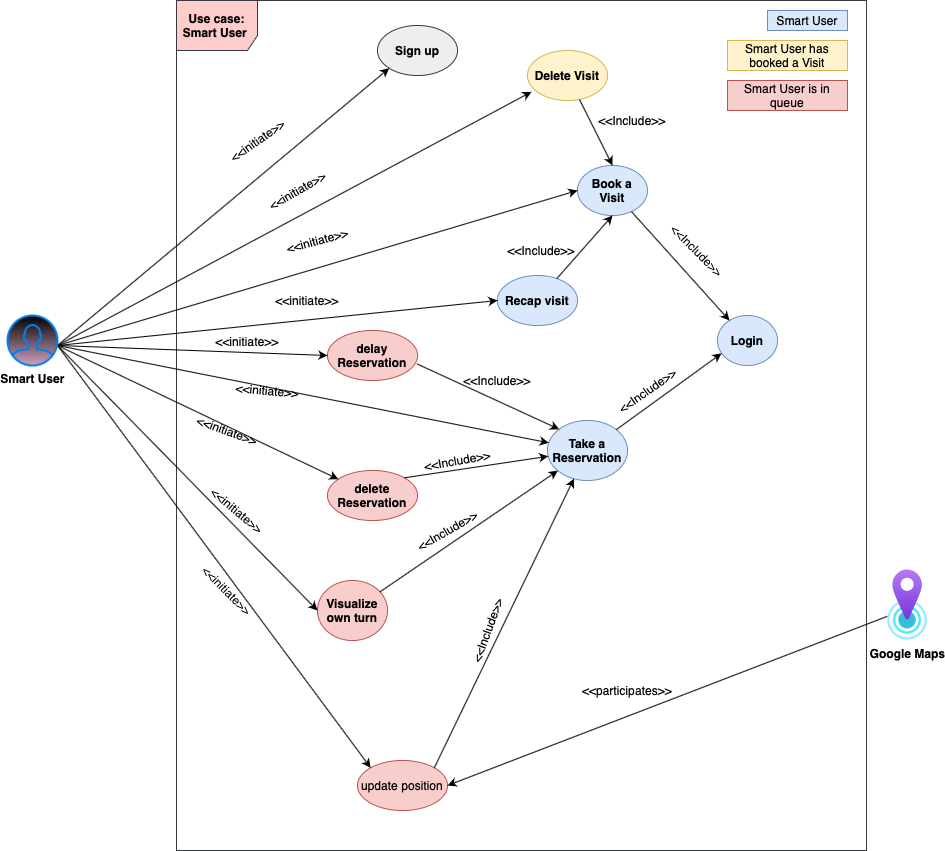
\includegraphics[scale=0.45]{diagrams/UseCaseUser.png}}
    \caption{Use case of the Smart User.}
\end{figure}

\pagebreak

\begin{table}[H]\begin{tabular}{|p{5cm} | p{7cm} | }
\hline
Name & \textbf{Login} \\
\hline
Actor & \textbf{Smart User} \\
\hline
Entry condition &
\begin{itemize}
\item User is already registered with his credential. 
\item User open the application.
\end{itemize} \\
\hline
Events flow & 
\begin{itemize}
	\item User open the application.
	\item The fields of username and password are filled by the User. 
	\item User send the request to the system by clicking "Login".
\end{itemize} \\
\hline
Exit condition & User is logged in and the homepage of CLup is provided. \\
\hline 
Exceptions &
\begin{itemize}
	\item Username inserted by the User is not registered in the system yet.
	\item Password inserted by the User is wrong.
    \item Communication with the Server is unavailable.
\end{itemize} \\
\hline
\end{tabular}

\caption{Login use case (smart User).}

\end{table}

\bigbreak
\begin{table}[H]\begin{tabular}{|p{5cm} | p{7cm} | }
	\hline
	Name & \textbf{Sign up} \\
	\hline
	Actor & \textbf{Smart User} \\
	\hline
	Entry condition &
	\begin{itemize}
		\item User open the application.
        \item User is not registered with his credential yet. 
	\end{itemize} \\
	\hline
	Events flow & 
	\begin{itemize}
		\item User selects “Create new account”.
		\item The fields of sensitive data, username and password are filled by the User.
		\item User accepts CLup privacy policy by checking its box.
		\item User clicks on "Register" button to send to the Server his request to be registered.
	\end{itemize} \\
	\hline
	Exit condition & \begin{itemize} 
    \item User is registered and already logged in. 
    \item CLup provides a page where User will select his market.
    \end{itemize}\\
	\hline 
	Exceptions &
	\begin{itemize}
		\item Username inserted by the User is already registered in the system.
		\item Userser did not accept CLup privacy policy.
		\item User has inserted forbidden characters in one or more fields.
        \item Communication with the Server is unavailable.
	\end{itemize} \\
	\hline
\end{tabular}
\caption{Use case of sign up (Smart User).}
\end{table}

\bigbreak

\begin{table}[H]\begin{tabular}{|p{5cm} | p{7cm} | }
	\hline
	Name & \textbf{Book a Visit} \\
	\hline
	Actor & \textbf{Smart User} \\
	\hline
	Entry condition &
	\begin{itemize}
		\item User has already logged in CLup with his credential.  
		\item User hasn't a Visit not yet submitted. 
	\end{itemize} \\
	\hline
	Events flow & 
	\begin{itemize}
		\item User clicks on "Homepage" option.
		\item User clicks “Book a visit” button.
		\item User selects the date and the time in which want to schedule the Visit.
		\item User chooses the shopping size of his grocery shopping.
		\item User confirms and sends the request to the Server by clicking "Next". 
	\end{itemize} \\
	\hline
	Exit condition & 	
    \begin{itemize}
    \item The user has booked his Visit.
    \item QRCode associated to the Visit is provided to the User. 
    \end{itemize}
 \\
	\hline 
	Exceptions & \begin{itemize}
		\item The time table choosen by the User is unavailable or already full.
        \item Communication with the Server is unavailable.
	\end{itemize}  \\ 
	\hline
\end{tabular}
\caption{Use case of Visit booking (Smart User).}
\end{table}

\bigbreak

\begin{table}[H]\begin{tabular}{|p{5cm} | p{7cm} | }
	\hline
	Name & \textbf{Take Reservation} \\
	\hline
	Actor & \textbf{Smart User} \\
	\hline
	Entry condition &
	\begin{itemize}
		\item User has already logged in CLup with his credential. 
		\item User hasn't a Reservation not yet submitted. 
	\end{itemize} \\
	\hline
	Events flow & 
	\begin{itemize}
		\item User clicks on "Homepage" option.
		\item User clicks “Reserve a seat” button.
		\item User confirms and sends the request to the Server by clicking "Yes".
	\end{itemize} \\
	\hline
	Exit condition &
	\begin{itemize}	
		\item User is inserted in the queue.
		\item QRCode associated to the Reservation is provided to the User. 
	\end{itemize} \\
	\hline 
	Exceptions & \begin{itemize}
    \item The market choosen is closed in the current moment of the request.
    \item Communication with the Server is unavailable.
    \end{itemize}
 \\
	\hline
\end{tabular}
\caption{Use case of Reservation booking (Smart User).}
\end{table}

\pagebreak

\begin{table}[H]\begin{tabular}{|p{5cm} | p{7cm} | }
	\hline
	Name & \textbf{Delete Visit} \\
	\hline
	Actor & \textbf{Smart User} \\
	\hline
	Entry condition &
	\begin{itemize}
		\item User has already logged in CLup with his credential. 
		\item User has already booked a Visit not yet submitted. 
	\end{itemize} \\
	\hline
	Events flow & 
	\begin{itemize}
		\item User clicks on “QRCode” menù.
		\item Visit and Reservation booked are provided.
		\item User clicks on “Delete” button of the Visit.
		\item User send the cancellation request to the Server by confirming it with "Yes".
	\end{itemize} \\
	\hline
	Exit condition &
	\begin{itemize}	
		\item The system deletes the User's Visit from his application.
		\item The system release the seat occupied in the slot/slots selected by the User's Visit.
	\end{itemize} \\
	\hline 
	Exceptions & Communication with the Server is unavailable. \\ 
	\hline
\end{tabular}
\caption{Use case of Visit delete (Smart User).}

\end{table}

\bigbreak


\begin{table}[H]\begin{tabular}{|p{5cm} | p{7cm} | }
	\hline
	Name & \textbf{Delete Reservation} \\
	\hline
	Actor & \textbf{Smart User} \\
	\hline
	Entry condition &
	\begin{itemize}
		\item User has already logged in CLup with his credential. 
		\item User has already booked a Reservation not yet submitted.
	\end{itemize} \\
	\hline
	Events flow & 
	\begin{itemize}
		\item User clicks on “QRCode” menù.
		\item Visit and Reservation booked are provided.
		\item User clicks on “Delete” button of the Reservation.
		\item User send the cancellation request to the Server by confirming it with "Yes".
	\end{itemize} \\
	\hline
	Exit condition &
	\begin{itemize}	
		\item The system deletes the User's Reservation from his application.
		\item The system release the seat occupied in the queue by the User.
	\end{itemize} \\
	\hline 
	Exceptions & Communication with the Server is unavailable.\\
	\hline
\end{tabular}
\caption{Delete Reservation use case (Smart User).}
\end{table}

\bigbreak

\begin{table}[H]\begin{tabular}{|p{5cm} | p{7cm} | }
	\hline
	Name & \textbf{Delay Reservation} \\
	\hline
	Actor & \textbf{Smart User}\\
	\hline
	Entry condition &
	\begin{itemize}
		\item User has already logged in CLup with his credential. 
		\item User has already booked a Reservation not yet submitted.
	\end{itemize} \\
	\hline
	Events flow & 
	\begin{itemize}
		\item User clicks on “QRCode” menù.
		\item Visit and Reservation booked are provided.
		\item User clicks on “Delay” button of the Reservation.
		\item User send the delay request to the Server by confirming it with "Yes", in order to go back in the queue by 10 seats.
	\end{itemize} \\
	\hline
	Exit condition &
	\begin{itemize}
		\item The user turn will be shift ten places after.
		\item The delay button will be disabled.
	\end{itemize} \\
	\hline 
	Exceptions & 
	\begin{itemize}
		\item Queue is too small for a delay.
		\item Delay option was already used by the User for this Reservation.
    	\item Communication with the Server is unavailable.
	\end{itemize} \\
	\hline
\end{tabular}
\caption{Delay Reservation use case (Smart User).}
\end{table}

\bigbreak

\begin{table}[H]\begin{tabular}{|p{5cm} | p{7cm} | }
	\hline
	Name & \textbf{Recap Visit} \\
	\hline
	Actor & \textbf{Smart User} \\
	\hline
	Entry condition &
    \begin{itemize}
	    \item User has already logged in CLup with his credential. 
		\item User has already booked a Visit not yet submitted.
        \end{itemize}\\
	\hline
	Events flow & \begin{itemize}
	\item User clicks on “QRCode” menù.
    \item User clicks on the QRCode of the Visit.
    \end{itemize}\\
	\hline
	Exit condition & CLup provided:
    \begin{itemize}
    \item QRCode;
    \item startTime of the Visit;
    \item endTime of the Visit;
    \end{itemize}\\
	\hline 
	Exceptions & \\
	\hline
\end{tabular}
\caption{Recap Visit use case (Smart User).}
\end{table}

\bigbreak

\begin{table}[H]\begin{tabular}{|p{5cm} | p{7cm} | }
	\hline
	Name & \textbf{Visualize turn in queue} \\
	\hline
	Actor & \textbf{Smart User} \\
	\hline
	Entry condition &
	\begin{itemize}
	    \item User has already logged in CLup with his credential. 
		\item User has already booked a Reservation not yet submitted.
        \end{itemize}\\
	\hline
	Events flow & 
	\begin{itemize}
	\item User clicks on “QRCode” menù.
    \item User clicks on the QRCode of the Reservation.
    \end{itemize} \\
	\hline
	Exit condition & CLup provided:
    \begin{itemize}
    \item QRCode;
    \item Number of people ahead the User in the queue;
    \item Time estimated to reach the market;
    \end{itemize} \\
	\hline 
	Exceptions & \\
	\hline
\end{tabular}
\caption{Use case of turn in queue visualization.}
\end{table}

\bigbreak

\begin{table}[H]\begin{tabular}{|p{5cm} | p{7cm} | }
	\hline
	Name & \textbf{Update position}  \\
	\hline
	Actor & \textbf{Smart User} \\
	\hline
	Entry condition &
	\begin{itemize}
	    \item User has already logged in CLup with his credential. 
		\item User has already booked a Reservation not yet submitted.
        \end{itemize} \\
	\hline
	Events flow & 
	\begin{itemize}
		\item User clicks on “QRCode” menù.
        \item User clicks on the QRCode of the Reservation.
        \item User clicks on "Update" botton.
	\end{itemize} \\
	\hline
	Exit condition &
	The system, through Google Maps, provided the time estimated to reach the market depending on his position. \\
	\hline 
	Exceptions & 
	\begin{itemize}
		\item The GPS position too far from market.
		\item GPS is unavailable.
	\end{itemize} \\
	\hline
\end{tabular}
\caption{Update position use case.}

\end{table}

\bigbreak

\begin{table}[H]\begin{tabular}{|p{5cm} | p{7cm} | }
	\hline
	Name & \textbf{Market selection}  \\
	\hline
	Actor & \textbf{Smart User} \\
	\hline
	Entry condition & User has already logged in CLup with his credential. \\
	\hline
	Events flow & 
	\begin{itemize}
		\item User selects the market in which wants to go grocery shopping.
		\item User confirms and sends his choice clicking on "Next". 
	\end{itemize} \\
	\hline
	Exit condition &
	The homepage of CLup is provided.  \\
	\hline 
	Exceptions & Communication with the Server is unavailable.\\
	\hline
\end{tabular}
\caption{Use case of market selection.}
\end{table}

\pagebreak

\subsection{Reception}
\par \medskip
{\normalsize \textbf{Scenario 3}}
\par \medskip
 Gustavo, an elderly person, he discovered recently a new time saver and usefull service at the market. \\
 It consists to book a visit at the market by simply calling the number found in an advertisment. \\
 Due to the fact that Gustavo is sick of waiting too much in the queue decide to call this market number to book the visit. \\
 On the other side Marta, a gentle receptionist who works for the market, answers to Gustavo's call; she takes care of the registration of his own data, the credentials and the all visit information (i.e data and range time).\\
Gustavo will be notified about the appointment with an SMS on his mobilephone in time. \\
In addition the SMS will provide the schedule for the visit and the code which will be submitted at the entrance.
 
\bigbreak

 
 
 \begin{figure}[H]
 	\caption{Use case of the Receptionist.}
 	
 	\centering
 	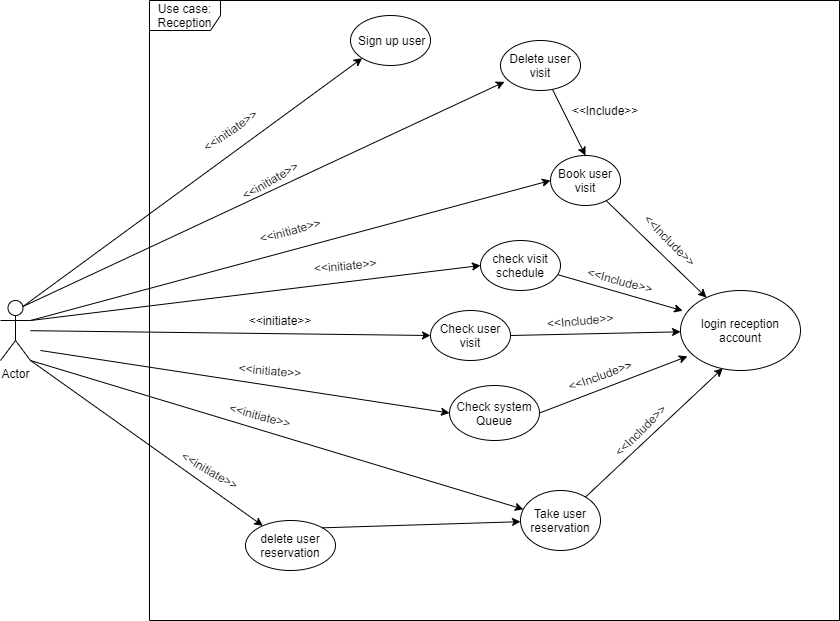
\includegraphics[scale = 0.40]{diagrams/UseCaseReception.png}
 	
 \end{figure}

\bigbreak
 
 \begin{table}[H]\begin{tabular}{|p{5cm} | p{7cm} | }
 	\hline
 	Name & \textbf{Sign up Mobile User}  \\
 	\hline
 	Actor & \textbf{Receptionist}  \\
 	\hline
 	Entry condition &
 	\begin{itemize}
 		\item Receptionist has already logged in CLup Operator. 
 		\item The Mobile User is not registered yet by a Receptionist.
        \item Mobile User calls the Receptionist to register himself.
 	\end{itemize} \\
 	\hline
 	Events flow & 
 	\begin{itemize}
 		\item Receptionist asks Mobile user the required sensitive data.
 		\item Receptionist fills the fields of the registration request.
 		\item Receptionist confirm and send the registration to the Server.
 	\end{itemize} \\
 	\hline
 	Exit condition &
 	The Mobile User is registered in the CLup system. \\
 	\hline 
 	Exceptions & 
 	\begin{itemize}
 		\item The phone call was aborted.
 	\end{itemize} \\
 	\hline
 \end{tabular}
\caption{Use case of sign up (Mobile User).}
 \end{table}
\bigbreak

\begin{table}[H]\begin{tabular}{|p{5cm} | p{7cm} | }
	\hline
	Name & \textbf{Delete Mobile User Visit}  \\
	\hline
	Actor & \textbf{Receptionist} \\
	\hline
	Entry condition &
	\begin{itemize}
        \item Receptionist has already logged in CLup Operator. 
 		\item Mobile User is already registered by a Receptionist.
		\item User has already booked a Visit not yet submitted. 
        \item Mobile User calls the Receptionist to delete his Visit.
	\end{itemize} \\
	\hline
	Events flow & 
	\begin{itemize}
		\item User provides his sensitive data to the Receptionist in order to be recognized by him. 
        \item Receptionist selects the Mobile User once he find him in th system.
		\item Receptionist has accessed to the booking's information of the Mobile User.
		\item Receptionist sends the cancellation request to the Server by clicking the “delete” button near the Visit.
	\end{itemize} \\
	\hline
	Exit condition & \begin{itemize}	
		\item The system deletes the User's Visit from his application.
		\item The system release the seat occupied in the slot/slots selected by the User's Visit.
	\end{itemize}\\
	\hline 
	Exceptions & 
	Communication with the Server is unavailable. \\
	\hline
\end{tabular}
\caption{Use case of Visit delete (Mobile User).}

\end{table}
\bigbreak

\begin{table}[H]\begin{tabular}{|p{5cm} | p{7cm} | }
	\hline
	Name & \textbf{Book Mobile User Visit}  \\
	\hline
	Actor & \textbf{Receptionist} \\
	\hline
	Entry condition &
	\begin{itemize}
		\item Receptionist has already logged in CLup Operator. 
 		\item Mobile User is already registered by a Receptionist.
		\item User hasn't a Visit not yet submitted. 
        \item Mobile User calls the Receptionist to book his Visit.
	\end{itemize} \\
	\hline
	Events flow & 
	\begin{itemize}
		\item User provides his sensitive data to the Receptionist in order to be recognized by him. 
        \item Receptionist selects the Mobile User once he find him in th system.
		\item Receptionist has accessed to the booking's information of the Mobile User.
        \item Recepetionist clicks on "Book" button near Visit.
		\item Receptionist selects the date and the time in which Mobile User wants to schedule the Visit.
		\item Receptionist chooses the shopping size of his grocery shopping.
		\item Receptionist confirms and sends the request to the Server by clicking "Next".
	\end{itemize} \\
	\hline
	Exit condition & \begin{itemize}
	\item The user has booked his Visit
    \item SMS is sent to the Mobile User with the string code and Visit schedule informations. 
    \end{itemize}\\
	\hline 
	Exceptions & 
	\begin{itemize}
    \item The time table choosen by the Mobile User is unavailable or already full.
    \item Communication with the Server is unavailable.
    \end{itemize} \\
	\hline
\end{tabular}
\caption{Book Visit use case (Mobile User).}
\end{table}
\bigbreak

\begin{table}[H]\begin{tabular}{|p{5cm} | p{7cm} | }
	\hline
	Name & \textbf{Take Mobile User Reservation} \\
	\hline
	Actor & \textbf{Receptionist} \\
	\hline
	Entry condition &
	\begin{itemize}
		\item Receptionist has already logged in CLup Operator. 
 		\item Mobile User is already registered by a Receptionist.
		\item User hasn't a Reservation not yet submitted. 
        \item Mobile User calls the Receptionist to delete his Reservation.
	\end{itemize} \\
	\hline
	Events flow & 
	\begin{itemize}
        \item User provides his sensitive data to the Receptionist in order to be recognized by him. 
        \item Receptionist selects the Mobile User once he find him in th system.
		\item Receptionist has accessed to the booking's information of the Mobile User.
        \item Receptionist sends the request to the Server by clicking on "book" button near Reservation.
	\end{itemize} \\
	\hline
	Exit condition &
	The user has been queued \\
	\hline 
	Exceptions & 
	The queue is full \\
	\hline
\end{tabular}
\caption{Use case of Reservation booking (Mobile User).}

\end{table}
\bigbreak

\begin{table}[H]\begin{tabular}{|p{5cm} | p{7cm} | }
	\hline
	Name & \textbf{Delete Mobile User Reservation} \\
	\hline
	Actor & \textbf{Receptionist} \\
	\hline
	Entry condition &
	\begin{itemize}
		\item Receptionist has already logged in CLup Operator. 
 		\item Mobile User is already registered by a Receptionist.
		\item User has a Reservation not yet submitted. 
        \item Mobile User calls the Receptionist to delete his Reservation.
	\end{itemize} \\
	\hline
	Events flow & 
	\begin{itemize}
		\item User provides his sensitive data to the Receptionist in order to be recognized by him. 
        \item Receptionist selects the Mobile User once he find him in th system.
		\item Receptionist has accessed to the booking's information of the Mobile User.
        \item Receptionist sends the request to the Server by clicking on "delete" button near Reservation.
	\end{itemize} \\
	\hline
	Exit condition & \begin{itemize}
	\item The system deletes the User’s Visit from his application.
    \item The system release the seat occupied in the slot/slots selected by the Mobile User’s Visit. \end{itemize} \\
	\hline 
	Exceptions & 
	The user has not booked any reservation \\
	\hline
\end{tabular}
\caption{Use case of Reservation delete (Mobile User).}
\end{table}
\bigbreak

\begin{table}[H]\begin{tabular}{|p{5cm} | p{7cm} | }
	\hline
	Name & \textbf{Login Receptionist account} \\
	\hline
	Actor & \textbf{Reception} \\
	\hline
	Entry condition &
	The receptionist opens CLup Operator on desktop device.  \\
	\hline
	Events flow & 
	\begin{itemize}
		\item Receptionist fills his credentials.
		\item Receptionist send the request to the Server to be authenticated and handle Mobile Users' booking by clicking "Login" button.
	\end{itemize} \\
	\hline
	Exit condition & \begin{itemize}
	\item The receptionist has logged in CLup Operator.
    \item CLup Operator provides the homepage where can handle bookings.
    \end{itemize}
    \\
	\hline 
	Exceptions & 
	\begin{itemize}
		\item Username inserted by the Receptionist is not registered in the system yet.
	    \item Password inserted by the Receptionist is wrong.
        \item Communication with the Server is unavailable.
	\end{itemize} \\
	\hline
\end{tabular}
\caption{Use case of Receptionist's login.}
\end{table}

\pagebreak

\subsection{Sequence Diagrams}
In this section are reported the main operation (Reservation and Visit) made by  Users to make an appointment in the market.\\
Note that are attached request of User with a Smartphone. Requests for Mobile Users are the same, with a difference: the presence of the actor Receptionist, who acts as a proxy in order to manage the requests.


\begin{figure}[H]
  \caption{Sequnce diagram of a Visit request from Smart User.}
  \label{fig:SD_visit}
  \centering
  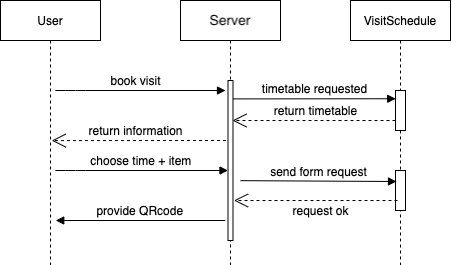
\includegraphics[scale=0.45]{diagrams/SD_visit.png}

\end{figure}
\begin{figure}[H]
  \caption{Sequnce diagram of a Reservation request from Smart User.}
  \label{fig:SD_reservation}
  \centering
  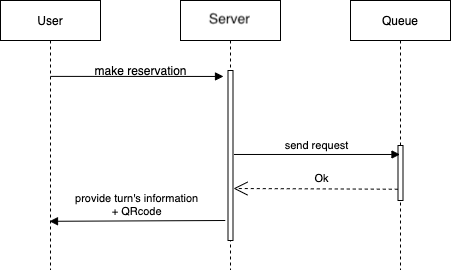
\includegraphics[scale=0.45]{diagrams/SD_reservation.png}

\end{figure}

\section{Performance Requirements}
The system has been designed to give possibility to Users to make and to manage their booking every time they need. So it's essential that the CLup's server have to handle a big number of connections. \\
The most reliable requests must be about the booking. User could book his appointment when he needs without any error or denial. 
Anyway there's one exception: the booking of a reservation is not avaialable when a market is closed.\\
It's important that the server has enough resources to accept a large number of request. The number will be estimated depending on the users demand.\\
\section{Design Constraints}
\subsection{Standards compliance}
Especially, the system will be released in the main digital distribution platform (such as App Store or Google Play). So it must follow their guidelines in order to have a proper and a lawful distribution. \\
In addition, due to the fact that it retrives and analyses many sensitive data, application must respect tha main privacy guidance. In particular in Europe must follow the General Data Privacy Regulation (GDPR), due to a safe and aware processing of data. 
\par
\subsection{Users in the market}
An important constraint that must applied is about the number of presences in the market of the Users. In fact, due to the Covid-19 pandemic, it's important that Users respect the social distance rule that is at least 1 meter.\\
So it's necessary that the market's provide the maximum number of Users allowed in the market that is, in a general way, it will be indicated with N.
\par
\subsection{Hardware limitations}
\begin{itemize}
\item 3G/4G/5G connection: they're essential due to server connection to compile booking request;
\item GPS: it's used to allow user to estimate the time spending to reach the market in time. But it's not mandatory for booking;
\end{itemize}
\subsection{Any other constraint}
\textbf{Mobile User telephone number}. Every Mobile User in the system provides at the registration many data but only one will be subject to a constraint: the telephone number. Indeed, the system memorize it, being for him the unique allowed to call the Receptionist for managing his booking. \par
The respective recognition made for a Smart User are their credential (e-mail and password).

\pagebreak

\section{Software System Attributes}
\subsection{Reliability}
The application will be tested for each update for verifying the stability and correctness.
Furthermore, will be scheduled a periodic maintenance to ensure the system operation.
To improve fault tolerance will be used a technique like \textbf{mirroring}.
 

\subsection{Availability}
Due to the fact that nowadays grocery shopping is avaiable almost all day, the availability of the system is very high. So the required availability is close to 99\%. \\
However, the reservation function has a lower avaibility because of the inability to book a seat in queue if the market is closed in some hours of the day. 
\subsection{Security}
Security is one of the most critical aspect of CLup. So User's sensitive data are stored safely in DBMS accessibile only by strict level of privilege.\\ 
In addition, communication towards the application server (like login or booking requests) are implemented using  HTTPS protocol, which, with TLS protocol, ensure the encryption of every packets. Another important risk that must by avoid is the Denial of Service, which occurs when the server is unavailable due to incoming traffic flooding from malevoulous Users.\\
So it's important that the Server mitigates this, by using for instance SYN cookies or any possible arrangements in order to allocate less resources if it's not necessary.
\subsection{Maintainability}
The application implementation must be oriented towards an high scalability in order to gurantee an efficient and cheaper maintenance. This could be done by using design patterns.
\subsection{Portability}
The system must be smoothly portable almost for the main smartphone on the market (i.e Android or iOS). So CLup must be distributed for the main mobile store (i.e App Store and Google Play), coding it with the main program languages such as Android or Swing. Instead, CLup Operator
%, the application used by receptionist to book visit and reservation of the Users not %registered, 
must be compatible with the main Operating system such as Windows and Mac OS X. 